\documentclass[%
 aip,
 jcp,
%jmp,%
%bmf,%
 sd,%
%rsi,%
 amsmath,amssymb,
%preprint,%
 reprint,%
%author-year,%
%author-numerical,%
]{revtex4-1}

\usepackage[colorlinks=true,allcolors=blue]{hyperref}
\usepackage{graphicx}
\usepackage{epstopdf}
\usepackage{dcolumn}
\usepackage{bm}
%\usepackage[mathlines]{lineno}
%\linenumbers\relax

\usepackage{xr-hyper}
\externaldocument{ITIC-supp}
\externaldocument[S-]{ITIC-supp}


\usepackage[latin1]{inputenc}
\usepackage{tikz}
\usetikzlibrary{shapes,arrows}

\usepackage{enumitem}


\begin{document}

\preprint{AIP/123-QED}

\title{Coexistence Calculation Using the Isothermal-Isochoric Integration Method}

\author{S. Mostafa Razavi}
\email{sr87@uakron.edu}
\affiliation{Department of Chemical and Biomolecular Engineering, The University of Akron, Akron, Ohio 44325, USA}

\author{Richard A. Messerly}
\email{richard.messerly@nist.gov}
\affiliation{Thermodynamics Research Center, National Institute of Standards and Technology, Boulder, Colorado 80305, USA}

\author{J. Richard Elliott}
\email{elliot1@uakron.edu}
\affiliation{Department of Chemical and Biomolecular Engineering, The University of Akron, Akron, Ohio 44325, USA}

\date{\today}

%%%RAM: Search for my comments with "RAM"
%%%RAM: 4/23/2018
% Italicized NVT throughout to be consistent with equations and subscripts, etc.

\begin{abstract}
In this work, an isothermal-isochoric integration (ITIC) method is proposed and tested as a viable method for vapor pressure calculation by molecular simulation. Several tests were carried out to validate the method which resulted in less than 1 \% deviation from NIST REFPROP values for reduced temperatures of less than 0.85. While consistency is achieved between the ITIC method, Gibbs Ensemble Monte Carlo (GEMC) method, and Grand Canonical Monte Carlo (GCMC) method when reduced temperatures of 0.6-0.85, the ITIC method is much more effective for vapor pressure calculations at reduced temperatures of 0.45-0.6, where relative deviations from experimental data are often quite large but important for practical applications. It is shown that computational efficiency for the complete temperature range is often served best by applying the ITIC method for the entire temperature range rather than applying Monte Carlo (MC) methods for part of the range. Furthermore, the ITIC method lends itself to application with molecular dynamics (MD) as well as MC, advancing the prospect of simulation results that are quantitatively consistent across software platforms.
\end{abstract}

\keywords{Vapor Pressure, Vapor Liquid Equilibria, Phase Diagram, Liquid Density}

\maketitle

\section{Introduction} \label{sec:introduction}
Phase coexistence determination is important when characterizing the physical properties of a chemical compound. Both the vapor pressure ($P^{\mathrm{sat}}$) and saturation liquid and vapor density ($\rho_{\mathrm{liq}}$ and $\rho_{\mathrm{vap}}$) provide sensitive measures of the quality provided by a particular force field. In principle, the computation of phase coexistence is a simple matter of equating pressures, temperatures, and chemical potentials between the coexisting phases. Nevertheless, accurate computation of phase coexistence by molecular simulation has posed challenges over the years. 
%RAM: Reviewer recommended that we include a reference for this statement.

The most straightforward method to compute phase transition in molecular simulation is to simply define an $NVT$ system (constant number of molecules, volume, and temperature) of sufficient size and overall density that an explicit interface is encountered. However this method often results in imprecise results. First order phase transitions exhibit a considerable free energy barrier between two phases due to interfacial free energies. For systems with large interfaces, this energy barrier increases. This often results in hysteresis, and phase transformation irreversibly proceeds beyond the coexistence point. \cite{Frenkel1996} 
%RAM: Reviewer recommended that we substitute free energy with Gibbs energy
%RAM: Reviewer thought that the energy barrier actually decreases for large interfaces. Maybe verify this.

Alternatively, there are methods for calculating phase coexistence while avoiding explicit interfaces. The Gibbs Ensemble Monte Carlo (GEMC) method \cite{Panagiotopoulos1987} is one of the most popular phase coexistence determination methods \cite{Paluch2008}.  The GEMC method requires particle exchange between two phases which leads to its major drawback ,i.e. insertion of particles in dense phases for large molecules. This problem is especially exacerbated  at low temperatures. The lowest temperatures that are typically available in the literature rarely extend below a reduced temperature ($T_r = T/T_c$, where $T_c$ is the critical temperature) of 0.6 \cite{Martin1998,Potoff2009}. However, common methods for industrial applications treat the temperature range from $T_r=0.45$ to critical point. The Peng-Robinson equation of state, for example, is valid for reduced temperatures as low as 0.45. \cite{Peng1976} To provide fundamental physical models that address issues with industrial applications, molecular simulations must address the entire temperature range of interest. 

As another alternative, Kofke \cite{Kofke1993b} developed a method called Gibbs-Duhem integration which makes use of the Clapeyron equation to numerically integrate and proceed along the saturation line starting from one single coexistence point. The Gibbs-Duhem method can solve the insertion problem, but it provides a limited extension beyond the starting coexistence point, and it relies on a second method to obtain the initial coexistence point. Ahunbay et al. \cite{Ahunbay2004} have applied this approach but their implementation has not been tested below a reduced temperature of 0.55.

As one more alternative, thermodynamic integration can provide a reliable solution for free energy calculation. In this method, a series of simulations are performed along a path that connects the state of interest to a system for which the free energy is known. One should be careful that the path does not include any type of phase change. For example, Elliott et al. \cite{Elliott1999a} applied an isochoric integration method to calculate vapor-liquid equilibria of square well spheres, demonstrating deficiencies in the preceding MC results.  For square well spheres, a convenient starting isotherm was the hard sphere limit, for which the thermodynamics are well represented by the Carnahan-Starling equation\cite{Carnahan1969a}. In this work, however, results are sought for soft potential models of arbitrary molecular shape, for which the infinite temperature limit is not convenient. 

In the proposed method, simulation points are used across an isotherm and along isochores, hence the name isothermal-isochoric (ITIC) was chosen. Because the approach to low temperatures proceeds along an isochore initialized at the high temperature (supercritical) isotherm, insertion is not a problem. In principle, there is no lower limit for the applicability of this method, except the triple point. Also, the data generated along the path of integration are valuable on their own merits, providing distinct insights about how well the molecular model is performing under conditions of high temperature and pressure. In other words, ITIC provides greater quality of characterization than MC methods at both higher temperatures and lower temperatures.

As another advantage, vapor pressure calculation using molecular dynamics is often perceived as an impractical approach \cite{Nieto-Draghi2015}. In this work, we will show the possibility of using molecular dynamics in the context of ITIC integration as a viable tool for vapor pressure calculation without a significant increase in computational effort compared to the typical approach of applying GEMC.
%RAM: Reviewer recommended we avoid saying "50%", since this would require more clear validation. Can we just say, "with similar computational effor" or "without a significant increase in computational effort compared to..."
%SMR(5/2/18): I used RAM's second suggestion
 
The presentation is initiated in Section~\ref{sec:ITIC-method} with a brief review of the thermodynamics underlying the integration method, including the manner in which characterizing the virial coefficients leads to simple but accurate coexistence determination. The approach is validated in Section~\ref{sec:NIST-VAL} by applying it to coexistence data available from the National Institute of Standards and Technology (NIST). Sensitivity of the method to the virial coefficients is explored in Section~\ref{sec:Bx-Sensitivity}. Section~\ref{sec:VirialCalc} provides recommendations for the most convenient and effective methods for characterizing the virial coefficients by molecular simulation. 
%RAM 4/23/18:
%We need a sentence describing Section V. Something like:
Section~\ref{sec:FSE} investigates the magnitude of finite size effects. 
Section~\ref{sec:SimDetail} and Section~\ref{sec:ExampleSim} demonstrate applications to molecular simulations and comparison between ITIC method and other methods of phase coexistance calculation.

\section{Isothermal-Isochoric Integration Method} \label{sec:ITIC-method}
For a single component system, Eq.~(\ref{eqn:eqn1}) must be satisfied at vapor-liquid phase equilibrium
\begin{equation}
\begin{array}{l} {T^{\mathrm{vap}} =T^{\mathrm{liq}} } \\ {P^{\mathrm{vap}} =P^{\mathrm{liq}} } \\ {G^{\mathrm{vap}} =G^{\mathrm{liq}} } \end{array} \label{eqn:eqn1}
\end{equation}
where $G$ represents Gibbs free energy, and superscripts ``vap" and ``liq" denote the vapor and liquid phases, respectively. As mentioned in Section~\ref{sec:introduction}, calculating free energy of a system using the ITIC integration method involves connecting the state of interest to a state of known free energy. In the case of phase equilibrium calculation, the state of interest is saturated liquid and the state of known free energy is an ideal gas. In order to go from saturated liquid to low densities we cannot directly pass through the two phase region. To overcome this problem we take an alternative path. First, the temperature of saturated liquid is increased to a supercritical temperature (isochore). Second, the supercritical state is rarefied to low densities (isotherm). It is worth mentioning that this method requires several separate simulations in the canonical ensemble (NVT) to provide enough data points on the paths for numerical integration to be accurate. Isochoric and isothermal pathways are shown in Fig.~\ref{fig:ITICpathway}. The first stage involves integrating internal energy, $U$, according to Eq.~(\ref{eqn:eqn6}) which is derived using Eqs.~(\ref{eqn:eqn2}-\ref{eqn:eqn5}):
\begin{equation}
U=kT^{2} \left( \frac{\partial \ln Q}{\partial T}\right) _{\mathrm N,\mathrm V}  \label{eqn:eqn2}
\end{equation}

\begin{equation}
A \left( N,V,T \right)=-kT \ln Q\left(N,V,T\right)
\label{eqn:eqn3}
\end{equation}
%RAM 4/23/18: Removed extra negative sign before kT^2
\begin{equation}
U=kT^{2} \left( \frac{\partial (-A/kT)}{\partial T} \right)_{N,V} =\frac{\partial \beta A}{\partial \beta }  \label{eqn:eqn4}
\end{equation}
%RAM: Included constant of integration
\begin{equation}
\beta A=\int U\mathrm{d} \beta + \mathrm{constant}  \label{eqn:eqn5}
\end{equation}

\begin{equation}
 \frac{A-A^{\mathrm{ig}} }{RT} =\int \left( U-U^{\mathrm{ig}} \right) \mathrm{d}\left( \frac{1}{RT} \right) \label{eqn:eqn6}
\end{equation}
where $V$ represents volume, $R$ is the gas constant, $k$ is the Boltzmann constant, $A$ is the Helmholtz energy, $Q$ is the canonical partition function, $\beta \equiv \frac{1}{kT}$, and superscript ``ig'' denotes the ideal gas. 
%RAM 4/23/18: 
%We might want a simple explanation for how we go from 5 to 6. Something like:
Eq. \ref{eqn:eqn6} is obtained from Eq. \ref{eqn:eqn5} by taking the difference between the real and ideal gas states (where the constants of integration cancel). Note that $k =\frac{R}{N_{\rm A}}$, where $N_{\rm A}$ is Avogadro's number.

The second stage consists in performing the following integration: 
\begin{equation}
\frac{A-A^{\mathrm{ig}}}{RT} =\; \int _{0}^{\rho }\frac{Z-1}{\rho } \; \mathrm{d}\rho \label{eqn:eqn7}
\end{equation}
where $\rho$ represents density and $Z$ is the compressibility factor $(Z \equiv \frac{P}{\rho RT})$.

Therefore, the Helmholtz energy departure function of the liquid phase is calculated by integrating $(Z-1)/\rho$ from zero to the saturated liquid
density of interest along the supercritical isotherm ($T^{\mathrm{IT}} \approx 1.2\,T_c$), added to the Helmholtz energy calculated by integrating internal energy departure function with
respect to $1/T$ along the saturated liquid density isochore from $T_{r} \approx 1.2$ to saturation temperature

\begin{equation}
\begin{array}{l}
{\frac{A^{\mathrm{liq}} -A^{\mathrm{ig}} }{RT}} 
\\ 
{=\; \int _{0}^{\rho _{\mathrm{liq}} }\frac{Z-1}{\rho } \; \mathrm{d}\rho \mathop{|}\nolimits_{T^{\mathrm{IT}}} +\int _{T^{\mathrm{IT}}}^{T^{\mathrm{\mathrm{sat}}}
}(U-U^{\mathrm{ig}} )\; \mathrm{d} \left(\frac{1}{RT} \right) \mathop{|}\nolimits_{\rho _{\mathrm{liq}}}}  
\end{array} 
\label{eqn:eqn8}
\end{equation}

The Gibbs energy criterion of phase equilibrium shown in Eq.~(\ref{eqn:eqn1}) can be rewritten in departure function form as shown in Eq.~(\ref{eqn:eqn9}).
%RAM: Reviewer wants a clear explanation regarding how we convert a constant P to constant V in Eq 9 and 10. This might explain his other question, where did ln(Z) come from?
\begin{equation}
\frac{G^{\mathrm{liq}} -G^{\mathrm{ig}} }{RT} =\frac{G^{\mathrm{vap}} -G}{RT} ^{\mathrm{ig}} \label{eqn:eqn9}
\end{equation}
which can be rearranged in terms of the Helmholtz energy departure function
%RAM: Included parentheses for ln(Z)
\begin{equation}
\begin{array}{l}
{\left(\frac{A^{\mathrm{liq}} -A^{\mathrm{ig}} }{RT} \right)_{T,V} +Z_{\mathrm{liq}} -1-\ln(Z_{\mathrm{liq}})} 
\\ 
{=\left(\frac{A^{\mathrm{vap}} -A^{\mathrm{ig}} }{RT} \right)_{T,V} +Z_{\mathrm{vap}} -1-\ln(Z_{\mathrm{vap}})}  
\end{array} 
\label{eqn:eqn10}
\end{equation}

Note that the $\ln(Z)$ terms in Eq.~(\ref{eqn:eqn10}) are introduced when converting Gibbs energy departure function at constant $T,P$ in Eq.~(\ref{eqn:eqn9}) to Helmholtz energy departure function at constant $T,V$ in Eq.~(\ref{eqn:eqn10}).

The value for $Z_{\mathrm{vap}}$ in Eq.~(\ref{eqn:eqn10}) can be approximated using a virial expansion truncated at the $B_3$ term

\begin{equation}
{Z_{\mathrm{vap}}} = 1 + {B_2}{\rho_{\mathrm{vap}}} + {B_3}\rho_{\mathrm{vap}}^2
\label{eqn:eqn11}
\end{equation}

Therefore, 
\begin{equation}
\begin{array}{l}{\left( {\frac{{{A^{\mathrm{vap}}} - {A^{\mathrm{ig}}}}}{{RT}}} \right)_{\mathrm{T,V}}} = \int_0^{{\rho _{\mathrm{vap}}}} {\frac{{Z - 1}}{\rho } \mathrm{d}\rho } \\ = \int_0^{{\rho
_{\mathrm{vap}}}} {\frac{{{B_2}{\rho _{\mathrm{vap}}} + {B_3}\rho _{\mathrm{vap}}^2}}{\rho_{\mathrm{vap}} } \mathrm{d}\rho_{\mathrm{vap}} } = {B_2}{\rho _{\mathrm{vap}}} + \frac{1}{2}{B_3}\rho _{\mathrm{vap}}^2\end{array} \label{eqn:eqn12}
\end{equation}

Substituting Eq.~(\ref{eqn:eqn11}) and Eq.~(\ref{eqn:eqn12}) in Eq.~(\ref{eqn:eqn10}) yields
\begin{equation}
\begin{array}{l}{\left( {\frac{{{A^{\mathrm{liq}}} - {A^{\mathrm{ig}}}}}{{RT}}} \right)_{\mathrm{T,V}}} + {Z_{\mathrm{liq}}} - 1 - \ln \left( \frac{P}{{{\rho _{\mathrm{liq}}}RT}} \right) \\ = {B_2}{\rho _{\mathrm{vap}}} +
\frac{1}{2}{B_3}\rho _{\mathrm{vap}}^2 + {B_2}{\rho _{\mathrm{vap}}} + {B_3}\rho _{\mathrm{vap}}^2 - \ln \left( \frac{P}{{{\rho _{\mathrm{vap}}}RT}} \right) \end{array}
 \label{eqn:eqn13}
\end{equation}

Rearranging Eq.~(\ref{eqn:eqn13}) gives
%RAM: 5/3 Reviewer suggested we use fraction instead of 1.5, since this suggests some sort of precision
\begin{equation}
\frac{{{A^{\mathrm{liq}}} - {A^{\mathrm{ig}}}}}{{RT}} + {Z_{\mathrm{liq}}} - 1 + \ln \left( \frac{{{\rho _{\mathrm{liq}}}}}{{{\rho _{\mathrm{vap}}}}} \right) = 2{B_2} {\rho _{\mathrm{vap}}} + \frac{3}{2}{B_3} \rho _{\mathrm{vap}}^2 \label{eqn:eqn14}
\end{equation}
which can be rearranged further to solve for ${\rho _V}$

\begin{equation}
\begin{array}{l}
{\rho _{\mathrm{vap}} = }
\\ 
{{\rho _{\mathrm{liq}}}\exp \left( {{{\left( {\frac{{{A^{\mathrm{liq}}} - {A^{\mathrm{ig}}}}}{{RT}}} \right)}_{\mathrm{T,V}}} + {Z_{\mathrm{liq}}} - 1 - 2{B_2} {\rho _{\mathrm{vap}}} - \frac{3}{2}{B_3} \rho _{\mathrm{vap}}^2}
\right) }  
\end{array}
\label{eqn:rhoV}
\end{equation}

Eq.~(\ref{eqn:eqn14}) (or Eq.~(\ref{eqn:rhoV})) is solved for vapor density using the fixed-point iteration method \cite{Burden1985} starting from an initial low value guess for $\rho_\mathrm{vap}$ and $Z_\mathrm{liq}$. Once vapor density is calculated, Eq.~(\ref{eqn:eqn16}) gives the vapor pressure.

\begin{equation}
P^\mathrm{sat} = P_\mathrm{vap} = {Z_\mathrm{vap}}{\rho _\mathrm{vap}}RT^\mathrm{sat} = (1 + {B_2} {\rho_\mathrm{vap}} + {B_3}\rho _\mathrm{vap}^2){\rho _\mathrm{vap}}RT^\mathrm{sat} 
\label{eqn:eqn16}
\end{equation}

Then, $Z_\mathrm{liq}$ is updated 
\begin{equation}
{Z_{\mathrm{liq}}} = \frac{P^\mathrm{sat}}{\rho_\mathrm{liq}RT}  
\label{eqn:zliq}
\end{equation}

$T^\mathrm{sat}$ is then updated by extrapolating the plot of $Z$ vs $1000/T$. Having new values for $T^\mathrm{sat}$, $Z_{\mathrm{liq}}$, and $\rho_\mathrm{vap}$, the next iteration can be started with Eq.~(\ref{eqn:rhoV}). However, $A^\mathrm{dep}$ should also be corrected since the value of $T^\mathrm{sat}$ is changed. Eq.~(\ref{eqn:aDepCorrection}) is used to serve this purpose. The iteration is stopped when the difference in two consecutive $\rho_\mathrm{vap}$ values are less than a defined tolerance. 

\begin{equation}
A^\mathrm{dep}_\mathrm{new} = A^\mathrm{dep} + \left( \frac{1}{T^\mathrm{sat}}-\frac{1}{T^\mathrm{IC}} \right) \frac{U^\mathrm{dep}T^\mathrm{sat}+U^\mathrm{dep}T^\mathrm{IC}}{2} 
\label{eqn:aDepCorrection}
\end{equation}

In order to obtain any saturation point, one needs to proceed through one isothermal and one isochoric path, to be able to calculate the free energy. The ITIC methodology was tested and validated using NIST Reference Fluid Properties (REFPROP) \cite{LEMMON-RP91} values by which the minimal number of data points on each path required to achieve reliable results was determined. In order to reach the densities of interest and maintain an acceptable accuracy to a reduced temperature of 0.45, one needs at least 9 data points on the isotherm and three data points on the isochore for each saturation point. The highest temperature state points, however, serve on both isochores and isotherm, hence these points are only simulated once. Therefore, a total of 19 state points are required to obtain 5 coexistence conditions. Fig.~\ref{fig:ITICpathway} provides a schematic plot of these state points. The isotherm is constructed at a supercritical temperature. A reduced temperature of $T_{r} \approx 1.2$ was the default value for the isotherm. For some compounds, owing to lack of NIST REFPROP values at high temperatures and the desire to compare isochores and isotherms to NIST REFPROP values when possible, a lower reduced temperature ($T_{r} \approx 1.05$) was chosen for the isotherm. Validations against NIST REFPROP values showed that any reduced temperature from 1.05 to 1.2 leads to acceptable accuracy.

\begin{figure}
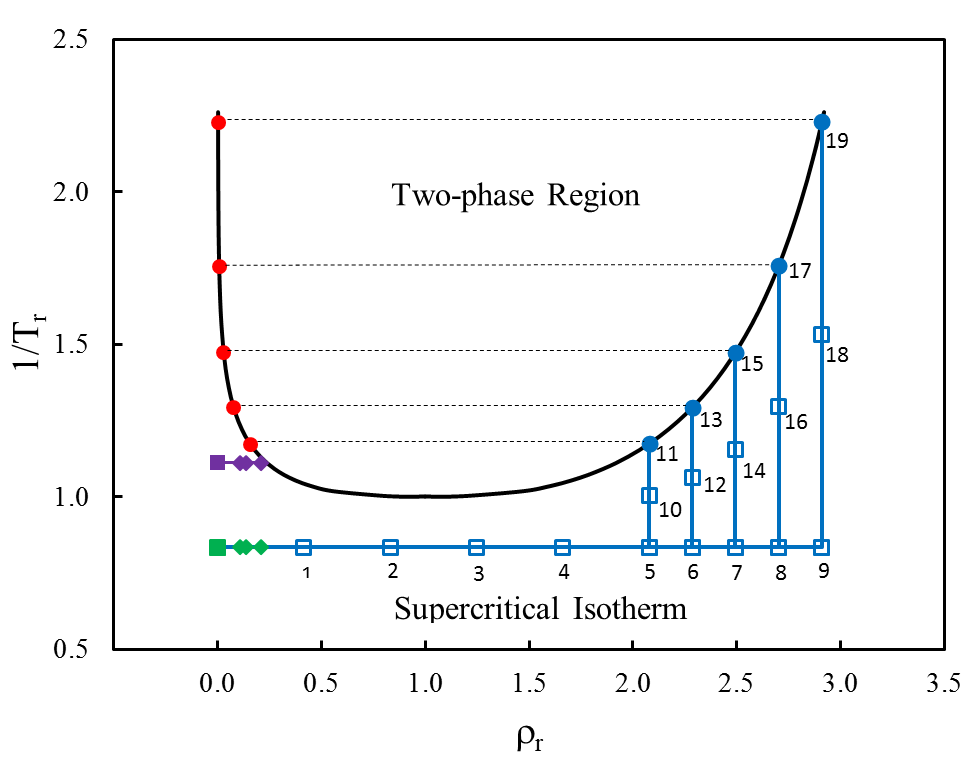
\includegraphics[scale=0.5]{Figures/ITIC-pathway-C2.png}
\caption{A schematic plot of the pathways taken in the ITIC method for ethane. The y-axis represents the reciprocal reduced temperature and the x-axis shows the reduced density. All the values were taken from NIST REFPROP \cite{Bucker2006}. Circles represent coexistence points while squares and diamonds represent non-saturated state points. Green and purple points show the state points required for $B_2$ calculation at isothermal temperature and $T_r=0.9$, respectively. }
\label{fig:ITICpathway}
\end{figure}

The integrations along the isotherm and isochores are performed using Simpson's rule \cite{atkinson2008}. Eq.~(\ref{eqn:eqn18}) and Eq.~(\ref{eqn:eqn19}) are
articulations of Simpson's rule used for numerical integration along the isotherm and isochores to calculate $A^{\mathrm{dep}}$ by Eq.~(\ref{eqn:eqn8}).

\begin{equation}
\int\limits_a^b {f(x)\mathrm{d} x \approx \frac{{b - a}}{6}} \left[ {f(a) + 4f \left( \frac{{a + b}}{2} \right) + f(b)} \right] \label{eqn:eqn18}
\end{equation}

\begin{equation}
\begin{array}{l}
{\int\limits_a^b f(x)\mathrm{d}x \approx }
\\ 
{{\frac{{b - a}}{8} \left[ {f(a) + 3f \left( \frac{{b - a}}{3} \right) + 3f \left( \frac{{2(b - a)}}{3} \right) + f(b)} \right]}}  
\end{array}
\label{eqn:eqn19}
\end{equation}

The $A^{\mathrm{dep}}$ values at points 2, 4, 7, and 9 in Fig.~\ref{fig:ITICpathway} are calculated using Eq.~(\ref{eqn:eqn18}) in which the value of function at three equidistant points on the x-axis are needed. The $A^{\mathrm{dep}}$ values at points 3, 5, and 8 are calculated using Eq.~(\ref{eqn:eqn19}) in which the value of the function at four equidistant points on the $x$ axis are needed. The $A^{\mathrm{dep}}$ at point 6 is equal to the integration value from point 6 to point 8 subtracted from the $A^{\mathrm{dep}}$ value at point 8. The $A^{\mathrm{dep}}$ value at point 1 is equal to the integration value from point 1 to point 4 subtracted from $A^{\mathrm{dep}}$ value at point 4. The green diamonds in Fig.~\ref{fig:ITICpathway} are used in estimating $B_2$ at isothermal temperature (green square) which is an essential part of ITIC integration. The purple diamonds are simulated to obtain a $B_2$ correlation for certain compounds for which $B_2$ at saturation temperatures were not available. The low density simulations (green diamonds and purple diamonds) are extrapolated to $\rho=0$ to estimate $B_2$. Note that the value of $(Z-1)/\rho$ at $\rho=0$ is equal to the second viral coefficient. This method is discussed in detail in Section \ref{sec:VirialCalc}. Figure~\ref{fig:algorithm} illustrates an algorithm starting from determining  ITIC state points to obtaining VLE properties.
%RAM: Converted all statements about Webbook to REFPROP

\begin{figure}[!h]
\centering
\tikzstyle{decision} = [diamond, draw, fill=blue!20, text width=6em, text badly centered, node distance=2cm, inner sep=0pt]
\tikzstyle{block} = [rectangle, draw, fill=blue!20, text width=20em, text centered, rounded corners, minimum height=1em]
\tikzstyle{block22} = [rectangle, draw, fill=blue!20, text width=22em, text centered, rounded corners, minimum height=1em]
\tikzstyle{block15} = [rectangle, draw, fill=blue!20, text width=15em, text centered, rounded corners, minimum height=1em]
\tikzstyle{smallblock} = [rectangle, draw, fill=blue!20, text width=8em, text centered, rounded corners, minimum height=1em]
\tikzstyle{line} = [draw, -latex']

\begin{tikzpicture}[node distance = 1cm, auto,thick,scale=0.8, every node/.style={scale=0.8}]
\node [block22] (pre1) {
\scriptsize Determine $\rho$ and $T$ values in Fig.~\ref{fig:ITICpathway}:
\begin{itemize}[]
\item \scriptsize Choose $\rho^9$, and calculate $\rho^{1-8}$
\item \scriptsize Estimate $T_\mathrm{sat}^\mathrm{est}$ values ($T^{11,13,15,17,19}$)
\item \scriptsize Calculate $T^{10,12,14,16,18}$
\item \scriptsize Choose $\rho$ for green ($T_\mathrm{IT}$) and purple ($T_\mathrm{0.9}$) points
\end{itemize}
};

\node [smallblock, below of=pre1,node distance=2.2cm] (step1) {\scriptsize Run NVT simulations};
\node [block,below of=step1,node distance=1cm] (step2) {\scriptsize Calculate $Z$, $U^\mathrm{dep}$ for all NVT simulations};
\node [block,below of=step2,node distance=1cm] (step2b) {\scriptsize Calculate $B_2^\mathbb{IT}$ (Eq.~\ref{eqn:Z1rhoB2B3}), and $B_2^\mathrm{sat}$ correlation (Section~\ref{sec:VirialCalc})};
\node [block,below of=step2b,node distance=1cm] (step3) {\scriptsize Pick an IC from Fig.~\ref{fig:ITICpathway} ($\rho_\mathrm{liq}=\rho^\mathrm{IC}$)};
\node [block,below of=step3,node distance=2cm] (step4) {\scriptsize Calculate $T^\mathrm{sat}_\mathrm{new}$ by extrapolating $Z$ vs. $1/T$ ($Z=Z_\mathrm{liq}$) };
\node [block,below of=step4,node distance=1cm] (step5a) {\scriptsize Calculate $A^\mathrm{dep}$ based on $T^\mathrm{sat}=T^\mathrm{sat}_\mathrm{est}$(Eq.~\ref{eqn:eqn8})};
\node [block,below of=step5a,node distance=1cm] (step5) {\scriptsize Correct $A^\mathrm{dep}$ (Eq.~\ref{eqn:aDepCorrection}) based on $T^\mathrm{sat}_\mathrm{new}$};
\node [block,below of=step5,node distance=1cm] (step6) {\scriptsize Calculate $\rho_\mathrm{vap}$ (Eq.~\ref{eqn:rhoV}), $P^\mathrm{sat}$(Eq.~\ref{eqn:eqn16})};
\node [decision,below of=step6,node distance=2.2cm] (step8) {\scriptsize $|\Delta\rho_\mathrm{vap}|<tol$?};
\node [block15,below of=step8,node distance=2.2cm] (step9) {\scriptsize Report $P^\mathrm{sat}$, $T^\mathrm{sat}$, $\rho_\mathrm{vap}$, and $\rho_\mathrm{liq}$ for IC};
\node [smallblock,left of=step8,node distance=4.5cm] (step7) {\scriptsize Update $Z_\mathrm{liq}$ (Eq.~\ref{eqn:zliq})};
\node [decision,below of=step9,node distance=2cm] (step10) {\scriptsize All IC's done?};
\node [smallblock,below of=step10,node distance=2cm] (step11) {\scriptsize Finish};

\path [line] (pre1) -- (step1);
\path [line] (step1) -- (step2);
\path [line] (step2) -- (step2b);
\path [line] (step2b) -- (step3);
\path [line] (step3) -- node {\scriptsize Set $Z_\mathrm{liq}=0.01$, $\rho_\mathrm{vap}=0.0$}(step4);
\path [line] (step4) -- (step5a);
\path [line] (step5a) -- (step5);
\path [line] (step5) -- (step6);
\path [line] (step6) -- (step8);
\path [line] (step8) -- node {no} (step7);
\path [line] (step8) -- node {yes}(step9);
\path [line] (step7) |- (step4);
\path [line] (step9) -- (step10);
\path [line] (step10) -- node {yes}(step11);
\path [line] (step10.east) -- +(3.5,0) |- node[pos=0.01] {no}(step3);

\end{tikzpicture}
\label{fig:algorithm}
\caption{Algorithm to obtain VLE from NVT simulations using ITIC method}
\end{figure}

\section{ITIC Validation}
\subsection{Validation using NIST REFPROP} \label{sec:NIST-VAL}
A simple way to test the accuracy of the ITIC method is to use a database that provides precise and self-consistent saturation properties and isochoric/isothermal properties. NIST Reference Fluid Properties (REFPROP) provides such values \cite{LEMMON-RP91,Bucker2006,Lemmon2004,Wagner2002}, which were used to validate the ITIC method. The following comparisons are solely based on NIST REFPROP equations, therefore the lack of statistical noise inherent to molecular simulation allows performing numerical integration very accurately. 

Fig.~\ref{fig:NIST-VALIDATION_C12_FTT_Psat} and Fig.~\ref{fig:NIST-VAL-C12-FTT_BINODAL} show the ITIC validation results for \textit{n}-dodecane when virial expansion in Eq.~(\ref{eqn:eqn11}) includes $B_{3}$ term. The deviations of calculated $P^{\mathrm{sat}}$, $\rho_{\mathrm{liq}}^{\mathrm{sat}}$, $\rho_{\mathrm{vap}}^{\mathrm{sat}}$, and $\Delta H_{\mathrm{v}}$ from the data obtained directly from NIST REFPROP \cite{Lemmon2004} are provided in Table \ref{tab:NIST-VAL-C12-FTT}. According to this table, one can reach a reduced saturation temperature ($T_r^{\mathrm{sat}}$) of 0.9 with less than 1 \% error in vapor pressure. The ITIC method fails to calculate accurate vapor pressure when $T_r^{\mathrm{sat}}>0.9$. If the $B_3$ term is excluded from Eq.~(\ref{eqn:eqn11}), the ITIC method fails for $T_r^{\mathrm{sat}} > 0.85$. Table~\ref{tab:NIST-VAL-C12-FTF} list the deviations from NIST REFPROP saturation data when $B_3$ is not used. As shown in this table, the ITIC method provides less than 1 \% deviation in vapor pressure when $T_r^{\mathrm{sat}} < 0.85$.

Fig.~\ref{fig:NIST-VALIDATION/C12/FTT/0_42690_rhov} illustrates the convergence paths taken by a fixed-point method to calculate $\rho_{\mathrm{vap}}$. Fig.~\ref{fig:NIST-VALIDATION/C12/FTF/0_42690_rhov} shows the same plot, except $B_3$ is excluded, i.e. virial expansion in Eq.~(\ref{eqn:eqn11}) is truncated at $B_{2}$ term. Using $B_3$ corrects the curve representing the right-hand side of Eq.~(\ref{eqn:rhoV}) ($g(\rho_{\mathrm{vap}})$) in such a way that fixed-point iteration converges. 

The vapor pressure was shown to be sensitive to the value of $B_3$ at saturation condition. This sensitivity and the sensitivity of vapor pressure to accuracy of $B_2$ at saturation temperatures as well as supercritical isothermal temperature is characterized in Section~\ref{sec:Bx-Sensitivity}.

\begin{figure} 
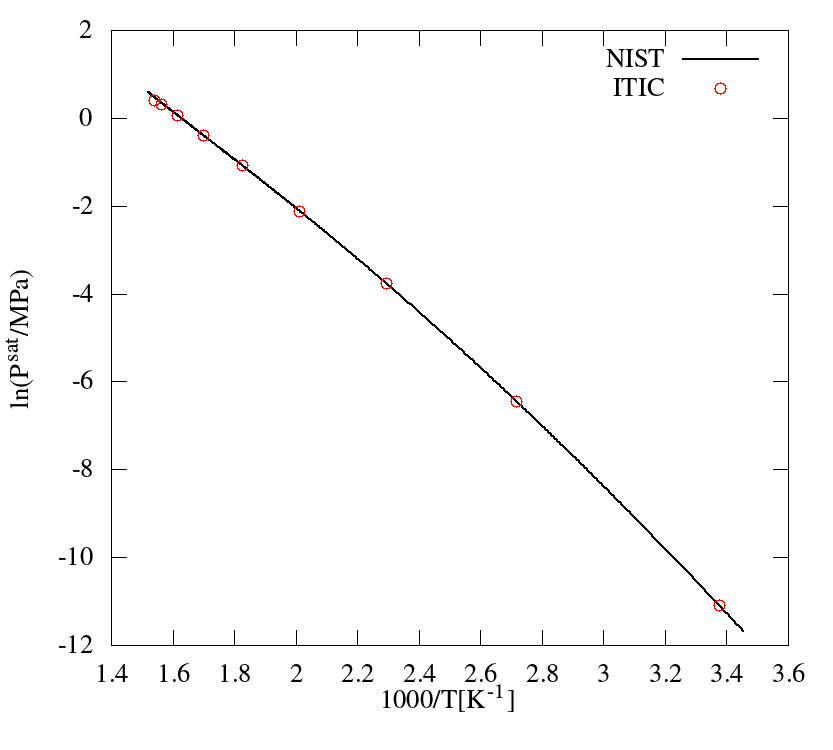
\includegraphics[scale=0.4]{Figures/NIST-VAL_FTT_psat.png}
\caption{$P^{\mathrm{sat}}$ plot of \textit{n}-dodecane. ITIC results are obtained using NIST REFPROP values \cite{Lemmon2004} for $U^{\mathrm{dep}}$ and $Z$. $B_3$ is included in Eq.~(\ref{eqn:rhoV}).}
\label{fig:NIST-VALIDATION_C12_FTT_Psat}
\end{figure}

\begin{figure}
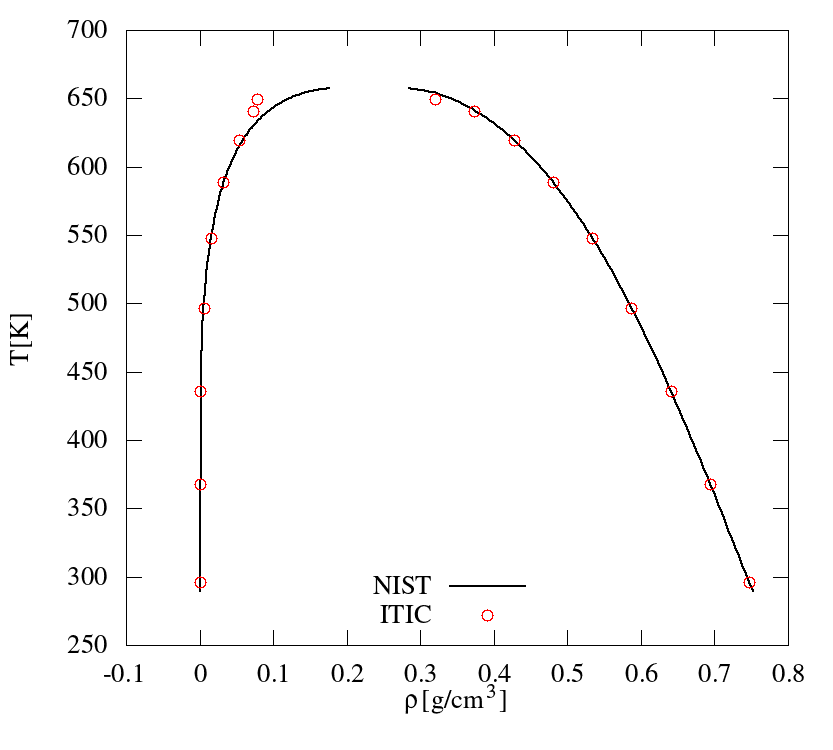
\includegraphics[scale=0.4]{Figures/NIST-VAL_FTT_trho.png}
\caption{Coexistence curves of \textit{n}-dodecane. ITIC results are obtained using NIST REFPROP values \cite{Lemmon2004} for $U^{\mathrm{dep}}$ and $Z$. $B_3$ is included in Eq.~(\ref{eqn:rhoV}).}
\label{fig:NIST-VAL-C12-FTT_BINODAL}
\end{figure}

\begin{figure} 
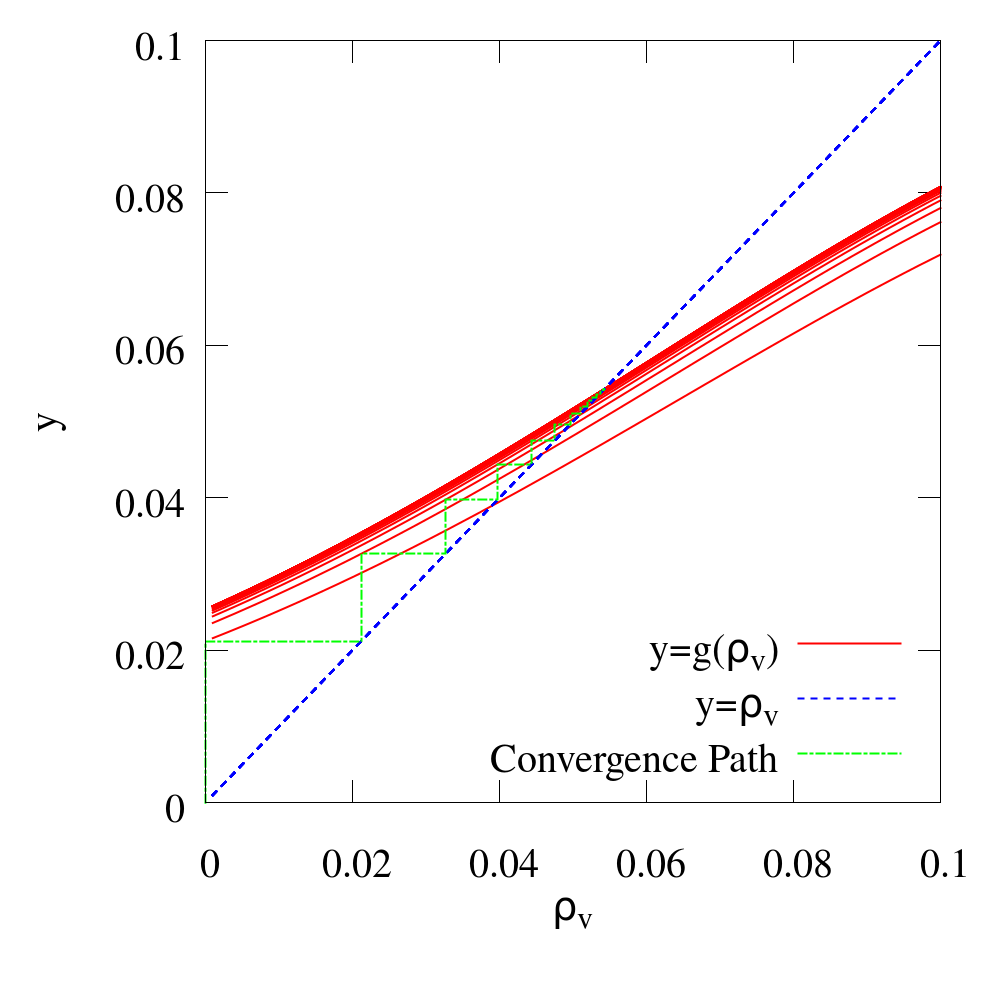
\includegraphics[scale=0.25]{Figures/NIST-VAL_FTT_C12_conv_0_42690.png}
\caption{Fixed-point method iteration and convergence path for \textit{n}-dodecane for the isochore corresponding to $\rho_{\mathrm{liq}}=0.4269\,\mathrm{g/cm^3}$ when $B_3$ is used in Eq.~(\ref{eqn:eqn11}). Eq.~(\ref{eqn:rhoV}) is summarized into $\rho_{\mathrm{vap}}=g(\rho_{\mathrm{vap}})$, i.e. the standard form of fixed-point method. The blue line represents the 45-degree line. The $g(\rho_{\mathrm{vap}})$ curves represent the right-hand side of Eq.~(\ref{eqn:rhoV}). At each iteration, $g(\rho_{\mathrm{vap}})$ is calculated based on a new set of $T^{\mathrm{sat}}$, $A^{\mathrm{dep}}_{\mathrm{L}}$, and $Z_{\mathrm{L}}$. Iteration starts with a low initial guess for $\rho_{\mathrm{vap}}$ and stops when absolute percent deviation between two consecutive $\rho_{\mathrm{vap}}$ values is less than a small tolerance, e.g. 0.1 \%.}
\label{fig:NIST-VALIDATION/C12/FTT/0_42690_rhov}
\end{figure}

\begin{figure} 
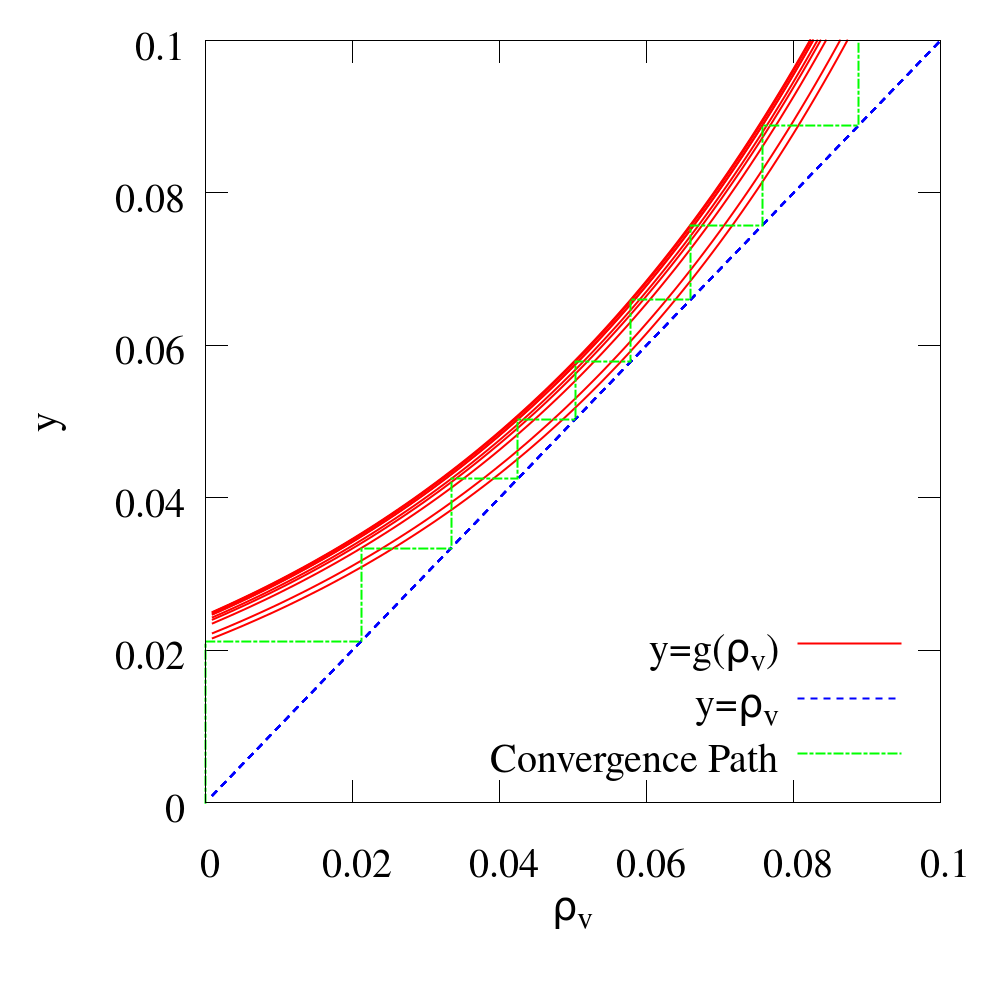
\includegraphics[scale=0.25]{Figures/NIST-VAL_FTF_C12_conv_0_42690.png}
\caption{Fixed-point method iteration and convergence path. The only difference between this figure and Fig.~\ref{fig:NIST-VALIDATION/C12/FTT/0_42690_rhov} is that $B_3$ term is excluded from Eq.~(\ref{eqn:eqn11})}
\label{fig:NIST-VALIDATION/C12/FTF/0_42690_rhov}
\end{figure}
%RAM: We should specify which compound Tables I-II refer to
\begin{table*}[]
\centering
\caption{Accuracy of the ITIC method for \textit{n}-dodecane when third virial coefficient is used}
\label{tab:NIST-VAL-C12-FTT}
\begin{ruledtabular}
\begin{tabular}{cccccccccc}
 & {[}K{]} &	 {[}MPa{]} &	 \% 	& {[}$\mathrm{g/cm^3}${]} & \% & {[}$\mathrm{g/cm^3}${]} & \% 	& {[}kJ/mol{]} & \% \\
$T_r^{\mathrm{sat}}$ & $T^{\mathrm{sat}}$ & $P^{\mathrm{sat}}$ & Dev.\footnote{Deviations are calculated using $\frac{\mathrm{ITIC - NIST}}{\mathrm{NIST}} \times 100$} & $\rho_{\mathrm{liq}}$ &	 Dev. & $\rho_{\mathrm{vap}}$ & Dev. & $\Delta H_{\mathrm{v}}$ & Dev. \\
\hline
0.987 & 649.33    & 1.5170088 & -6.08   & 0.3202     & -7.19   & 0.078389        & -34.28  & 15.63        & 19.06   \\
0.973 & 640.48    & 1.3808947 & -3.70   & 0.3736     & -0.80   & 0.072090        & -22.69  & 18.97        & 11.09   \\
0.942 & 619.73    & 1.0598150 & -1.53   & 0.4269     & -0.02   & 0.054262        & -8.37   & 24.15        & 3.09    \\
0.895 & 588.88    & 0.6788865 & -0.28   & 0.4803     & 0.03    & 0.032482        & -1.57   & 30.46        & 1.36    \\
0.833 & 548.06    & 0.3423508 & -0.07   & 0.5336     & 0.01    & 0.015427        & -0.26   & 36.89        & 0.95    \\
0.755 & 496.92    & 0.1206953 & 0.03    & 0.5870     & 0.01    & 0.005419        & 0.01    & 43.04        & 0.52    \\
0.663 & 436.21    & 0.0234394 & -0.08   & 0.6404     & 0.00    & 0.001129        & -0.08   & 48.99        & 0.19    \\
0.559 & 368.12    & 0.0015922 & 0.09    & 0.6937     & 0.00    & 0.000089        & 0.10    & 55.06        & 0.04    \\
0.450 & 296.21    & 0.0000153 & 0.46    & 0.7471     & 0.00    & 0.000001        & 0.89    & 61.76        & 0.01    \\ 			
\end{tabular}
\end{ruledtabular}
\end{table*}

\begin{table*}[]
\centering
\caption{Accuracy of the ITIC method for \textit{n}-dodecane when third virial coefficient is not used. For $T_r^{\mathrm{sat}}>0.9$ the fixed-point iteration does not converge.}
\label{tab:NIST-VAL-C12-FTF}
\begin{ruledtabular}
\begin{tabular}{cccccccccc}
 & {[}K{]} &	 {[}MPa{]} &	 \% 	& {[}$\mathrm{g/cm^3}${]} & \% & {[}$\mathrm{g/cm^3}${]} & \% 	& {[}kJ/mol{]} & \% \\
$T_r^{\mathrm{sat}}$ & $T^{\mathrm{sat}}$ & $P^{\mathrm{sat}}$ & Dev. & $\rho_{\mathrm{liq}}$ &	 Dev. & $\rho_{\mathrm{vap}}$ & Dev. & $\Delta H_{\mathrm{v}}$ & Dev. \\
\hline
0.935 & 615.05 & -2.5523492 & -353.51 & 0.3202 & -26.60 & 0.172892 & 220.25 & 1.20  & -95.14 \\
0.942 & 619.6  & -2.7091311 & -352.18 & 0.3736 & -12.56 & 0.177782 & 200.99 & 2.64  & -88.74 \\
0.928 & 610.4  & -1.4359029 & -252.54 & 0.4269 & -4.04  & 0.150039 & 204.09 & 9.18  & -64.22 \\
0.895 & 589.1  & 0.7097525  & 3.89    & 0.4803 & 0.10   & 0.040847 & 23.28  & 28.90 & -3.70  \\
0.833 & 548.07 & 0.3448984  & 0.65    & 0.5336 & 0.02   & 0.015851 & 2.46   & 36.77 & 0.61   \\
0.755 & 496.92 & 0.1208125  & 0.13    & 0.5870 & 0.01   & 0.005436 & 0.33   & 43.03 & 0.49   \\
0.663 & 436.21 & 0.0234409  & -0.08   & 0.6404 & 0.00   & 0.001129 & -0.06  & 48.99 & 0.19   \\
0.559 & 368.12 & 0.0015922  & 0.09    & 0.6937 & 0.00   & 0.000089 & 0.10   & 55.06 & 0.04   \\
0.450 & 296.21 & 0.0000153  & 0.46    & 0.7471 & 0.00   & 0.000001 & 0.89   & 61.76 & 0.01  \\
\end{tabular}
\end{ruledtabular}
\end{table*}

\subsection{Vapor Pressure Sensitivity to Virial Coefficients} \label{sec:Bx-Sensitivity}
In order to estimate the required accuracy of the second virial coefficient at the isothermal temperature (i.e. $(Z-1)/\rho$ at $\rho=0$), Fig.~\ref{fig:FTF-B2xX-IT-C12-Psat} was generated by changing $B_2$ and calculating the corresponding deviations in \textit{n}-dodecane vapor pressure. For example, $P^{\mathrm{sat}}$ changes by around 5 \% if $B_2$ at isotherm changes by 20 \%, and a 5 \% change in $B_2$ results in around 2 \% deviation in \textit{n}-dodecane's $P^{\mathrm{sat}}$. The sensitivity is almost independent of saturation reduced temperatures ($T_r^{\mathrm{sat}}$). This shows that it is imperative to use an accurate $B_2$ value at the isothermal temperature.

Vapor pressure precision is very weakly influenced at low temperatures by accuracy of the second and third virial coefficients in Eq.~(\ref{eqn:rhoV}) and Eq.~(\ref{eqn:eqn16}). Fig.~\ref{fig:FTF-B2xX-C12-Psat} shows the $P^{\mathrm{sat}}$ sensitivity to $B_2$ at various reduced temperatures, each representing one isochore. The first three lowest temperatures, are barely sensitive to $B_2$ precision such that even 50 \% error in $B_2$ results in less than 1 \% deviation in $P^{\mathrm{sat}}$. However, a relatively accurate $B_2$ is required to obtain accurate $P^{\mathrm{sat}}$ when $T_r>0.75$. Similarly, at $T_r=0.84$ one needs to stay below 2 \% deviation in $B_2$ in order to have less that 1 \% error in vapor pressure.

Above a certain reduced temperature (around 0.85), as illustrated in Fig.~\ref{fig:Diverge-C12-FTF-B2+15_rho-048030gcc}, the ITIC method fails to converge when $B_3$ is neglected. This leads to the unusual behavior of the $T_r=0.89$ plot in Fig.~\ref{fig:FTF-B2xX-IT-C12-Psat} and \ref{fig:FTF-B2xX-C12-Psat}. This upper limit can be increased by using the $B_3$ term in Eq.~(\ref{eqn:rhoV}) and Eq.~(\ref{eqn:eqn16}) which will help the $\rho_{\mathrm{vap}}$ to converge, as can be seen in Fig.~\ref{fig:Converge-C12-FTT-B3+15-rho_048030gcc}.

Fig.~\ref{fig:FTT-B3xX-C12-Psat} was plotted similar to Fig.~\ref{fig:FTF-B2xX-C12-Psat}, except $B_3$ term was added. It is worth mentioning that in order to truly understand the influence of $B_3$, exact values of $B_2$ were used from NIST REFPROP. Even though adding $B_3$ improves the overall behavior of fixed-point iteration in terms of convergence (Fig.~\ref{fig:NIST-VALIDATION/C12/FTT/0_42690_rhov} and Fig.~\ref{fig:NIST-VALIDATION/C12/FTF/0_42690_rhov}), the sensitivity of $P^{\mathrm{sat}}$ to $B_3$ is negligible when $T_r$ is less than 0.85. This supports the idea of setting the $B_3$ term to zero without significant loss of precision at such temperatures. 

\begin{figure}
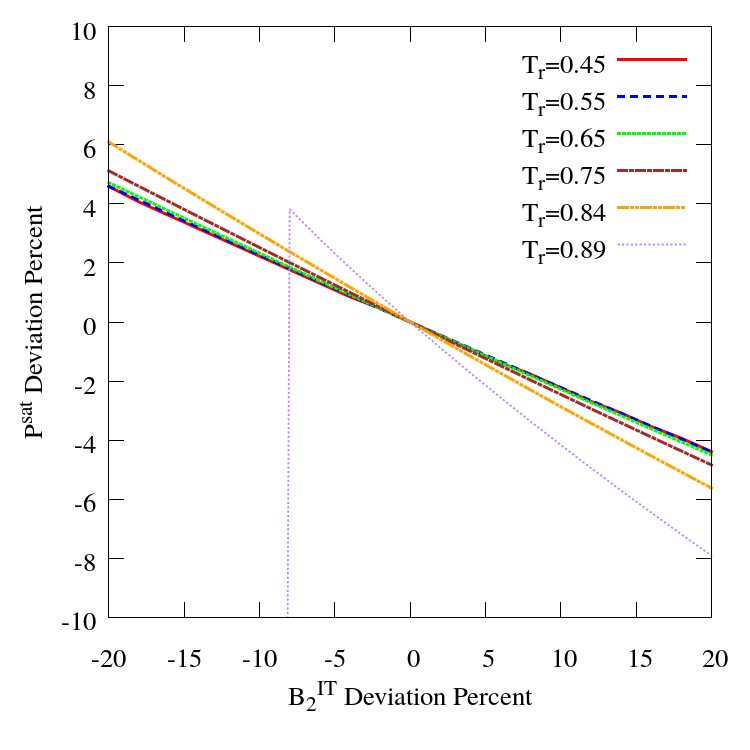
\includegraphics[scale=0.30]{Figures/FTF-B2xX-IT-C12-Psat.png}
\caption{$P^{\mathrm{sat}}$ sensitivity to isotherm $B_2$}
\label{fig:FTF-B2xX-IT-C12-Psat}
\end{figure}


\begin{figure}
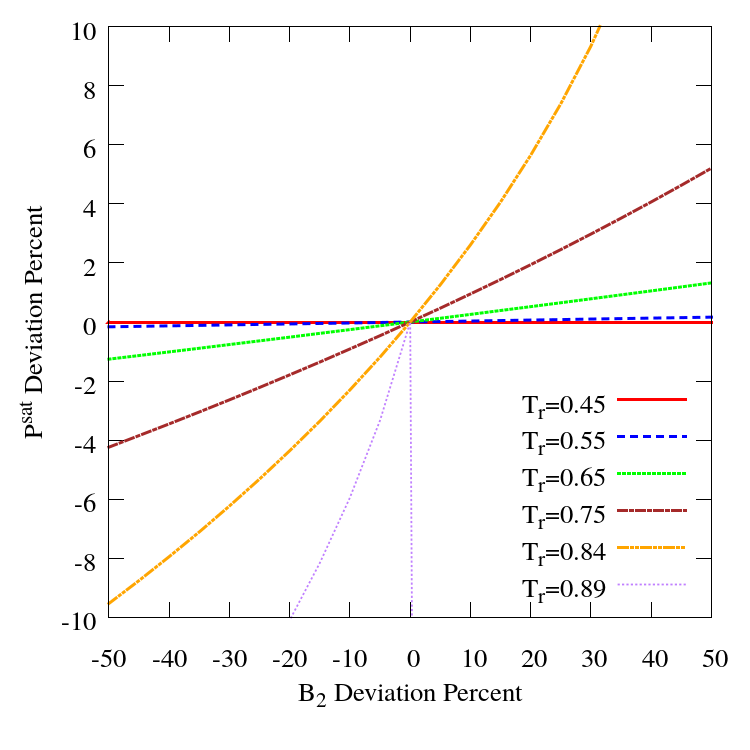
\includegraphics[scale=0.30]{Figures/FTF-B2xX-C12-Psat.png}
\caption{$P^{\mathrm{sat}}$ sensitivity to second virial coefficient used in Eq.~(\ref{eqn:eqn16})}
\label{fig:FTF-B2xX-C12-Psat}
\end{figure}

\begin{figure}
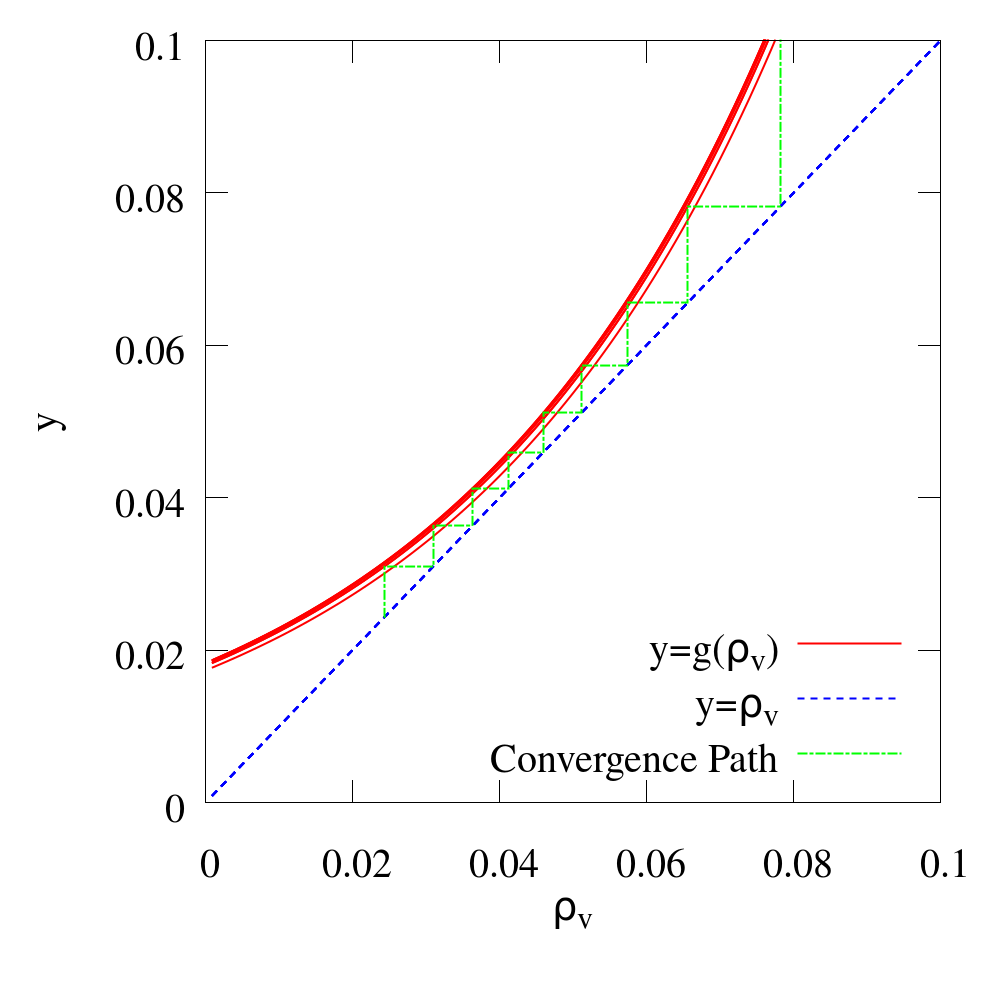
\includegraphics[scale=0.25]{Figures/Diverge-C12-FTF-B2+15_rho-048030gcc.png}
\caption{Fixed-point iteration path at reduced temperature of $T_r=0.89$. In this case, $B_2$ is not sufficient and $B_3$ is required.}
\label{fig:Diverge-C12-FTF-B2+15_rho-048030gcc}
\end{figure}

\begin{figure}
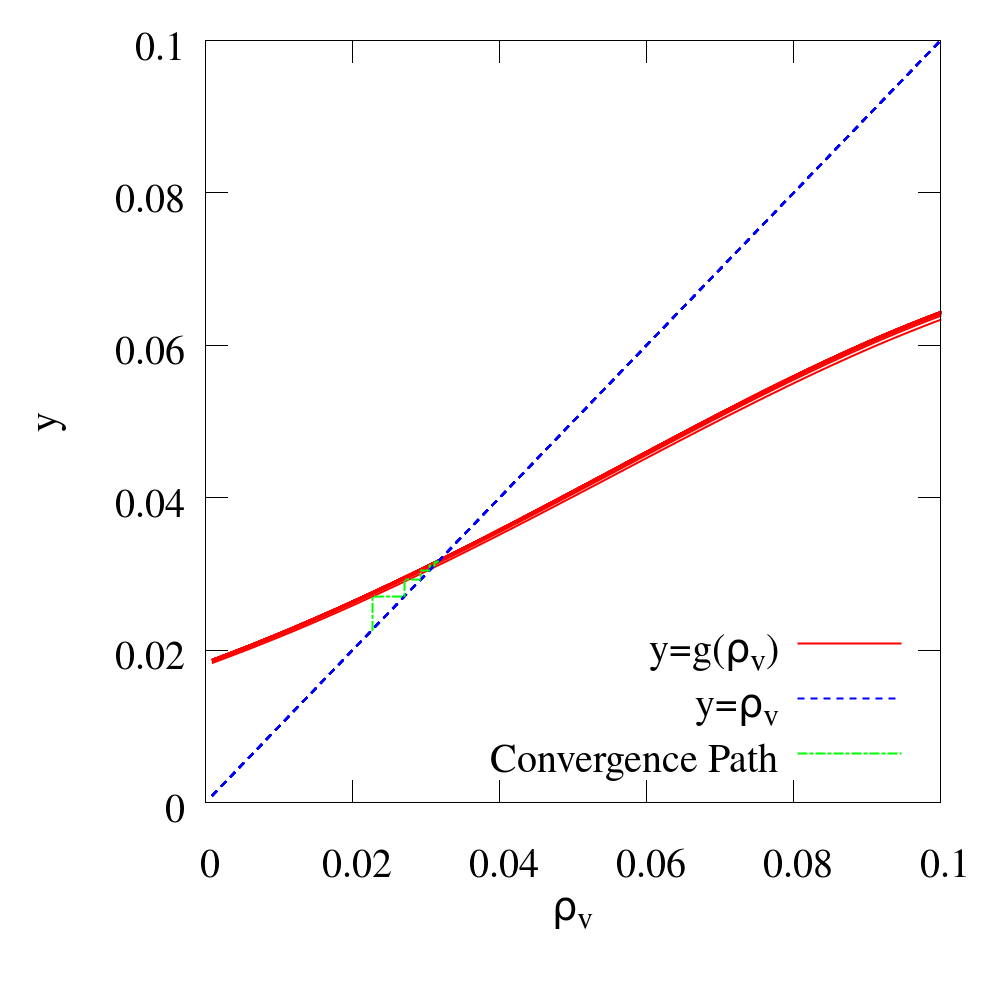
\includegraphics[scale=0.25]{Figures/Converge-C12-FTT-B3+15-rho_048030gcc.png}
\caption{Convergence path at reduced temperature of $T_r=0.89$. $B_3$ term helps the fixed-point iteration to converge.}
\label{fig:Converge-C12-FTT-B3+15-rho_048030gcc}
\end{figure}

\begin{figure}
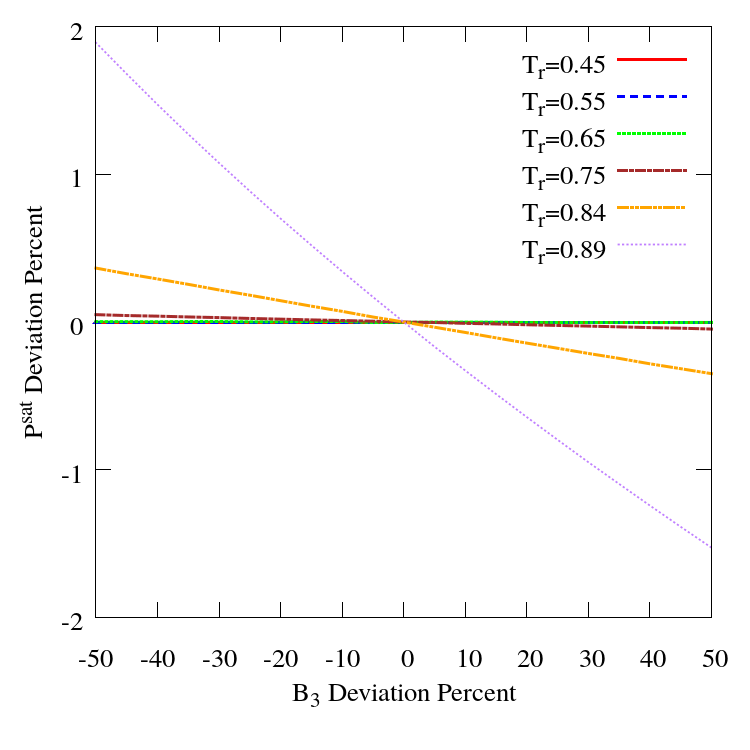
\includegraphics[scale=0.3]{Figures/FTT-B3xX-C12-Psat.png}
\caption{$P^{\mathrm{sat}}$ sensitivity to third virial coefficient used in Eq.~(\ref{eqn:eqn16})}
\label{fig:FTT-B3xX-C12-Psat}
\end{figure}


\section{Virial Coefficients Calculation} \label{sec:VirialCalc}
Second virial coefficients can be estimated by calculating the intercept of $(Z-1)/\rho$ with respect to $\rho$. In principle, the slope of this line at zero density gives the third virial coefficient. Fig.~\ref{fig:TraPPE-C2-Z1rho} shows the accuracy of this method when used at various temperatures. The intercept and slope of the blue lines in this figure represent Schultz's \cite{Schultz2010a} values of $B_2$ and $B_3$, respectively. These lines are plotted using Eq.~(\ref{eqn:Z1rhoB2B3})

\begin{equation}
\frac{Z-1}{\rho} = B_2 + B_3\rho \label{eqn:Z1rhoB2B3}
\end{equation}

It is shown for TraPPE-UA ethane that at temperatures above $T_r=0.80$, $B_2$ values calculated using this method are consistent with values reported by Schultz. At the two lowest temperatures in Fig.~\ref{fig:TraPPE-C2-Z1rho} the highest density point is not in line with the blue lines due to being in the two-phase region, therefore using the first three points for those temperatures gives a more accurate estimate of $B_2$ (green triangle).  

\begin{figure}
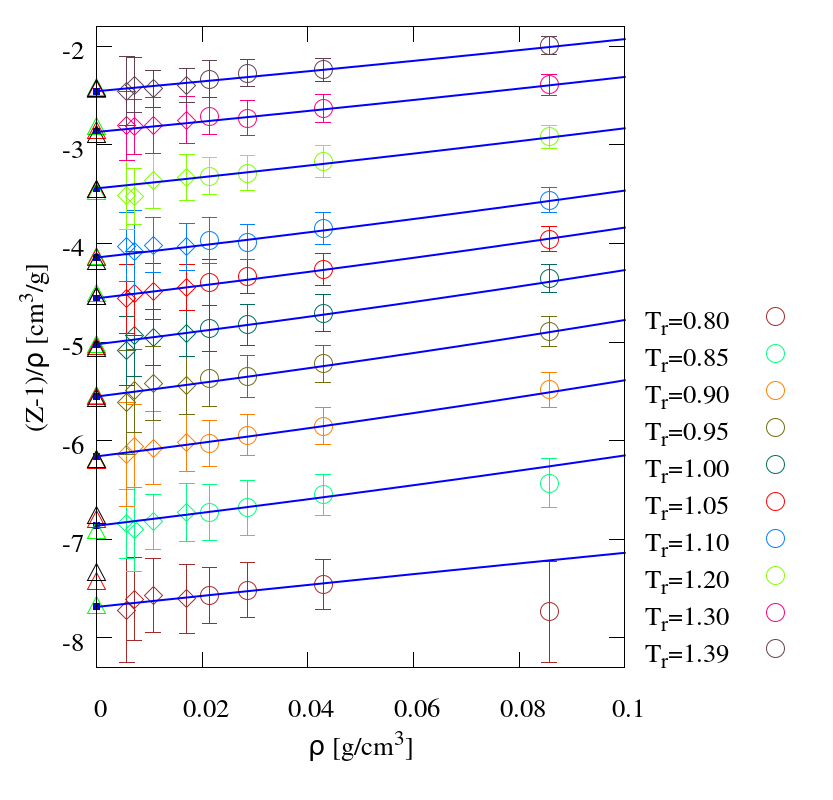
\includegraphics[scale=0.3]{Figures/TraPPE-C2-Z1rho.png}
\caption{Plot of $(Z-1)/\rho$ with respect to $\rho$ for ethane. Blue solid points represent Schultz's $B_2$ values in Ref.~\onlinecite{Ahunbay2004}. Each blue line represents Schultz values of intercept ($B_2$) and slope ($B_3$) at corresponding temperatures. Circles and diamonds are $NVT$ state points simulated in GOMC (GPU Optimized Monte Carlo) package \cite{Mick2013}. Diamond points are very low density simulations that were not used in $B_2$ and $B_3$ calculations. Black, green, and red triangles represent $B_2$ values estimated using Eq.~(\ref{eqn:Z1rhoB2B3}) when all four, first three, or last three state points were used, respectively.}
\label{fig:TraPPE-C2-Z1rho}
\end{figure}

\begin{figure}
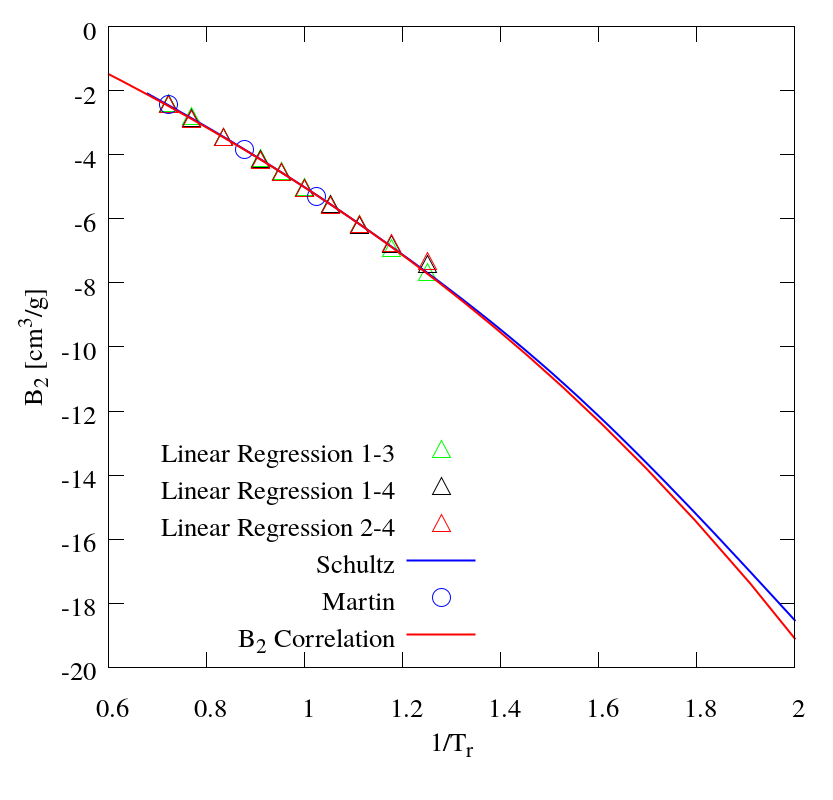
\includegraphics[scale=0.3]{Figures/TraPPE-C2-B2.png}
\caption{Second virial coefficient calculated with various methods. Black, red, and green triangles are $B_2$ values calculated using 1-4, 2-4, and 1-3 linear regressions, respectively. 1-4, 1-3, or 2-4 mean all four, first three, or last three state points were used in calculating $B_2$. The blue circles represent $B_2$ values obtained by Martin and Siepmann \cite{Martin1998} using a Monte Carlo method \cite{Harismiadis1994}. $B_2$ correlation is in good agreement with Schultz's simulation results \cite{Schultz2010a}.}
\label{fig:TraPPE-C2-B2}
\end{figure}

\begin{figure}
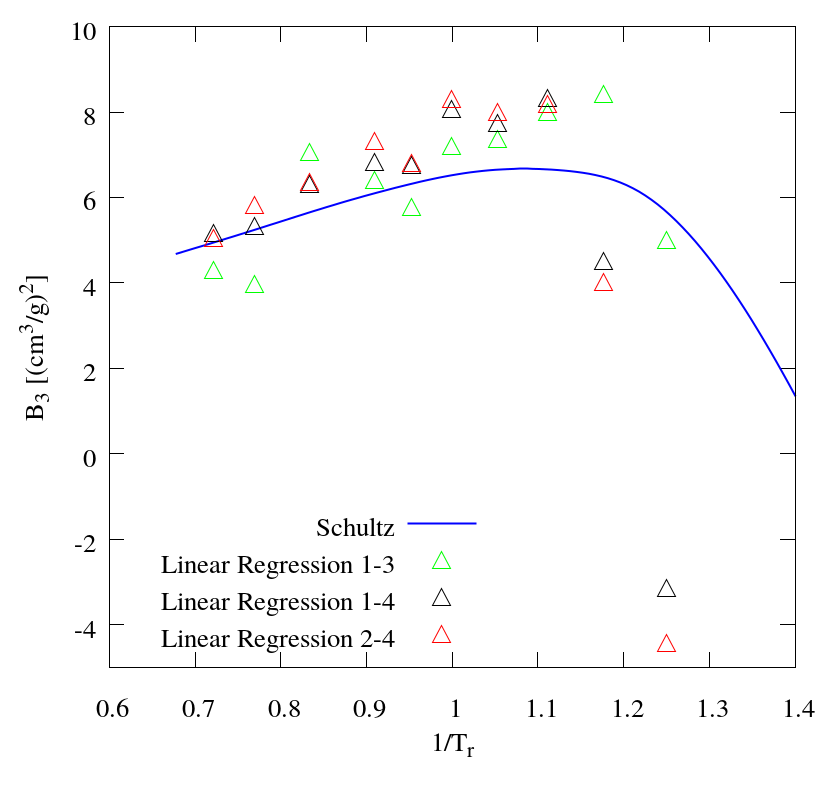
\includegraphics[scale=0.3]{Figures/TraPPE-C2-B3.png}
\caption{Third virial coefficient calculated with various methods}
\label{fig:TraPPE-C2-B3}
\end{figure}

According to Eq.~(\ref{eqn:rhoV}), it is important to have a correlation for $B_2$ and $B_3$ with respect to temperature, because temperatures change after each iteration and updated values for $B_2$ and $B_3$ are needed. In order to obtain such a correlation, the formula used in the DIPPR \cite{DIPPR2004} database was adapted, except the last term was removed to decrease the number of parameters and avoid overfitting, as shown in Eq.~(\ref{eqn:b2form}) 

\begin{equation}
B_2=A+\frac{B}{T}+\frac{C}{T^3} \label{eqn:b2form}
\end{equation}

Taking the derivative of $B_2$ with respect to $\beta$ leads to the internal energy departure function, as shown in  Eq.~(\ref{eqn:b2uDep})

\begin{equation}
\rho \frac{\beta \partial B_2}{\partial \beta}=\rho \left( \frac{B}{T}+\frac{3C}{T^3}\right)=\frac{U-U^{\mathrm{ig}}}{RT} \label{eqn:b2uDep}
\end{equation}

Eq.~(\ref{eqn:b2it}) and Eq.~(\ref{eqn:b2TrPoint9}) are obtained by inserting $B_2$ values extrapolated using Eq.~(\ref{eqn:Z1rhoB2B3}) and their corresponding temperatures into Eq.~(\ref{eqn:b2form}). 

\begin{equation}
B_2(T_{\mathrm{IT}})=A+\frac{B}{T_{\mathrm{IT}}}+\frac{C}{T_{\mathrm{IT}}^3} \label{eqn:b2it}
\end{equation}

\begin{equation}
B_2(T_{0.9})=A+\frac{B}{T_{0.9}}+\frac{C}{T_{0.9}^3} \label{eqn:b2TrPoint9}
\end{equation}
where $T_{0.9}$ is the temperature corresponding to reduced temperature of 0.9 and $T_{0.9}$ represents the isothermal temperature. 

Subtracting Eq.~(\ref{eqn:b2TrPoint9}) from Eq.~(\ref{eqn:b2it}) gives


\begin{equation}
B_2(T_{\mathrm{IT}})-B_2(T_{0.9})=B \left( \frac{1}{T_{\mathrm{IT}}}-\frac{1}{T_{0.9}} \right) +C \left( \frac{1}{T_{\mathrm{IT}}^3}-\frac{1}{T_{0.9}^3} \right) \label{eqn:b2subtract}
\end{equation}

The intercept of $\frac{U-U^{\mathrm{ig}}}{\rho RT}$ with respect to $\rho$ gives the value of $\beta \frac{\partial B_2}{\partial \beta}$

\begin{equation}
\beta \frac{\partial B_2}{\partial \beta}=\frac{B}{T_{0.9}}+\frac{3C}{T_{0.9}^3} \label{eqn:b2pB2pBeta}
\end{equation}

Solving three equations (Eq.~(\ref{eqn:b2it}), (\ref{eqn:b2subtract}), and (\ref{eqn:b2pB2pBeta})) with three unknowns gives the values of A, B, and C, hence a correlation for $B_2$ with respect to temperature is derived. Fig.~\ref{fig:TraPPE-C2-B2} shows a correlation obtained by this method. 

This method is successful for $B_2$ calculations, however $B_3$ calculation using Eq.~(\ref{eqn:Z1rhoB2B3}) is less accurate, as shown in Fig.~\ref{fig:TraPPE-C2-B3}. Fortunately, according to Fig.~\ref{fig:FTT-B3xX-C12-Psat} and Fig.~\ref{fig:FTF-B2xX-IT-C12-Psat}, it is not important to obtain an accurate value of $B_3$ as long as the value of $(Z-1)/\rho$ is accurately represented.

\section{Finite Size Effects}\label{sec:FSE}
According to Fig.~\ref{fig:FTF-B2xX-IT-C12-Psat}, $P^{\mathrm{sat}}$ accuracy is sensitive to accuracy of $B_2$ values at isothermal temperature ($B_2^{\mathrm{IT}}$). This sensitivity is due to accumulation of errors when integrating along isotherm, such that an error in $B_2^{\mathrm{IT}}$ affects the $A^{\mathrm{dep}}$ values at all other points along the isotherm and isochores. Similarly, one would expect a significant influence from low density points, i.e. points 1, 2, and 3 in Fig.~(\ref{fig:ITICpathway}). Therefore, it is imporatnt to investigate the factors affecting the accuracy of $Z$ at low densities on isotherm. The factors considered in this study are system size, the choice of MD or MC, and the choice of fixed bonds or flexible bonds. 

The system size effects at low densities are demonstrated in Fig.~\ref{fig:FSE_TraPPE_C2_Lammps_rigid_IT}-\ref{fig:FSE_TraPPE_C2_GOMC_IT}. Plot of $(Z-1)/\rho$ with respect to $\rho$ shown in Fig.~\ref{fig:FSE_TraPPE_C2_Lammps_rigid_IT} demonstares the effect of varying number of molecules in MD simulation of ethane in canonical ensemble. In order to match the $B_2+B_3 \rho+B_4 \rho^2$ line which represents the exact values of $(Z-1)/\rho$, we need 3200 ethane molecules to achieve low enough uncertainties for accurate extrapolation of $B_2$ for the simulation times chosen. In this plot C-C bonds are held constant using SHAKE algorithm \cite{Ryckaert1977}. 

The effect of using flexible bonds is shown in Fig.~\ref{fig:FSE_TraPPE_C2_Lammps_flex_IT}. The systematic discrepency from exact values (black line) as well as large uncertainties suggests that we should avoid flexible bonds at very low densities. A major problem with MD simulations with flexible bonds is the large pressure and energy fluctuations leading to the need for long equilibration and production times.
%RAM: Included GOMC reference here since only cited previously in caption fo Fig. 11
Fig.~\ref{fig:FSE_TraPPE_C2_GOMC_IT} shows the low density $NVT$ state points simulated using GOMC (GPU Optimized Monte Carlo) package \cite{Mick2013}. This plot shows that MC method gives more reliable results than MD for low density $NVT$ state points. Table~\ref{tab:FSE} compares the uncertainties of $Z$ when using different simulation methods. $\mathrm{STD}_1$ represents the average of four relative standard deviations of $Z$ (i.e., $\mathrm{STD}/Z\times100 \, \%$), each calculated during a single run, while $\mathrm{STD}_2$ is the relative standard deviation of $Z$ from four separate runs. According to this table, the standard deviation from four replicate simulations ($\mathrm{STD}_2$) are much smaller than the average standard deviation for a single run ($\mathrm{STD}_1$). Therefore, Fig.~\ref{fig:FSE_TraPPE_C2_Lammps_rigid_IT}-\ref{fig:FSE_TraPPE_C2_GOMC_IT} were plotted based on $\mathrm{STD}_2$ uncertainties. Table~\ref{tab:FSE} also shows that MC results have a much smaller $\mathrm{STD}_1$ and $\mathrm{STD}_2$ than rigid or flexible MD results. 

Therefore, we recommend using MC when simulating these low density points. The choice of MD or MC for other high density state points in ITIC method shown in Fig.~\ref{fig:ITICpathway} is less important, because they generally agree with each other within their uncertainties. In this study, we used MC for all state points. 

\begin{table*}[ht]
\centering
\caption{Compressibility factor and uncertainty at low densities. $\mathrm{STD}_1$ represents the average of four relative standard deviations each calculated during the corresponding individual runs, while $\mathrm{STD}_2$ is the relative standard deviation of $Z$ from four separate runs.}
\label{tab:FSE}
\begin{ruledtabular}
\begin{tabular}{cc|cc|cc|cc|cc}
       &        & \multicolumn{2}{c}{N=120} & \multicolumn{2}{c}{N=400} & \multicolumn{2}{c}{N=1600} & \multicolumn{2}{c}{N=3200} \\
Method & $\rho [\mathrm{g/cm^3}]$ & $\mathrm{STD}_1 \%$  & $\mathrm{STD}_2 \%$ & $\mathrm{STD}_1 \%$  & $\mathrm{STD}_2 \%$ & $\mathrm{STD}_1 \%$  & $\mathrm{STD}_2 \%$  & $\mathrm{STD}_1 \%$  & $\mathrm{STD}_2 \%$ \\
\hline
MC-rigid    & 0.0214 & 1.05   & 0.10 & 0.62   & 0.05 & 0.46  & 0.05 & -     & -    \\
MC-rigid    & 0.0286 & 1.27   & 0.11 & 0.69   & 0.06 & 0.55  & 0.06 & -     & -    \\
MC-rigid    & 0.0429 & 1.60   & 0.17 & 0.96   & 0.00 & 0.76  & 0.11 & -     & -    \\
MC-rigid    & 0.0857 & 2.54   & 0.23 & 1.59   & 0.08 & 1.38  & 0.17 & -     & -    \\
MC-rigid    & 0.1714 & 4.54   & 0.26 & 3.16   & 0.26 & 2.91  & 0.30 & -     & -    \\
MC-rigid    & 0.2571 & 6.55   & 0.60 & 4.62   & 0.63 & 4.32  & 0.25 & -     & -    \\
\hline
MD-rigid    & 0.0214 & 11.71  & 0.94 & 6.31   & 0.72 & 3.20  & 2.41 & 2.30  & 0.10 \\
MD-rigid    & 0.0286 & 13.56  & 1.02 & 7.33   & 0.16 & 3.80  & 4.78 & 2.60  & 0.11 \\
MD-rigid    & 0.0429 & 17.30  & 0.76 & 9.46   & 0.53 & 4.79  & 2.45 & 3.23  & 0.20 \\
MD-rigid    & 0.0857 & 28.35  & 1.14 & 15.01  & 0.36 & 7.49  & 0.39 & 5.15  & 0.36 \\
MD-rigid    & 0.1714 & 49.89  & 1.53 & 25.46  & 1.73 & 13.56 & 0.55 & 9.15  & 0.64 \\
MD-rigid    & 0.2571 & 65.65  & 2.44 & 35.96  & 0.75 & 18.38 & 0.52 & 12.57 & 0.47 \\
\hline
MD-flexible & 0.0214 & 106.25 & 1.39 & 59.51  & 0.88 & 29.67 & 0.78 & 19.12 & 0.56 \\
MD-flexible & 0.0286 & 113.52 & 2.01 & 61.35  & 0.45 & 30.83 & 0.66 & 20.39 & 0.59 \\
MD-flexible & 0.0429 & 129.34 & 3.16 & 65.61  & 0.71 & 35.84 & 0.32 & 22.10 & 0.34 \\
MD-flexible & 0.0857 & 152.29 & 2.52 & 83.85  & 1.15 & 42.60 & 1.20 & 27.49 & 0.33 \\
MD-flexible & 0.1714 & 196.67 & 2.49 & 101.51 & 2.90 & 53.94 & 0.82 & 38.10 & 0.46 \\
MD-flexible & 0.2571 & 227.96 & 0.94 & 125.42 & 1.28 & 58.77 & 1.60 & 42.61 & 0.87
\end{tabular}
\end{ruledtabular}
\end{table*}
%RAM: Fig 14-16 need [cm^3/g] on the y-axis
\begin{figure}
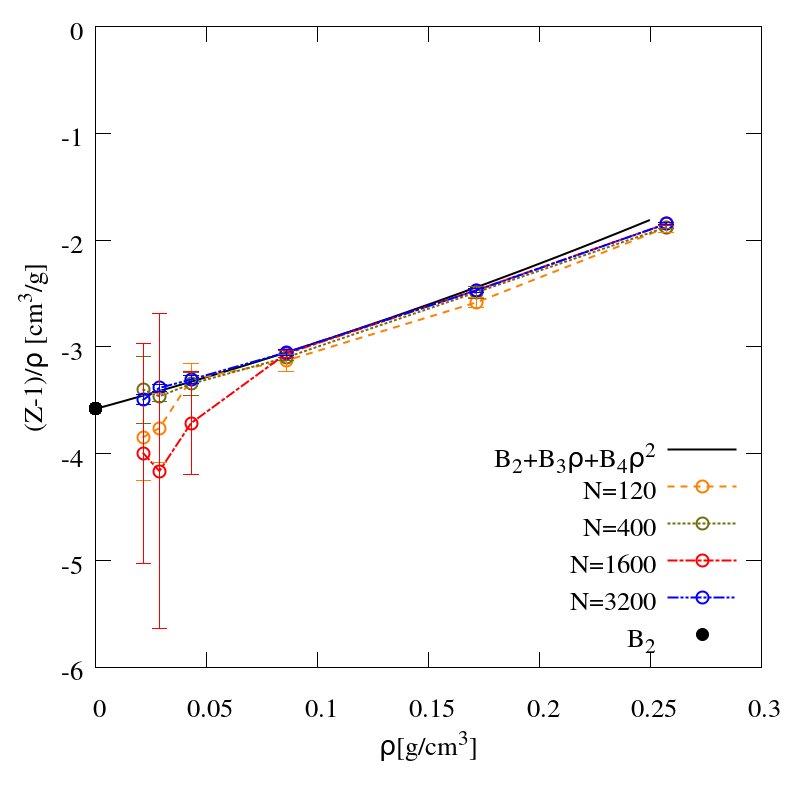
\includegraphics[scale=0.3]{Figures/FSE_TraPPE-C2_Lammps-rigid_IT.png}
\caption{Effect of number of ethane molecules on compressibility factor at low densities in MD simulation ($T^{\mathrm{IT}}=360 \, \mathrm{K}$). State points are simulated in LAMMPS with SHAKE algorithm to keep the C-C bond constant. Solid black line represents $B_2+B_3 \rho+B_4 \rho^2$ line where $B_{2-4}$ are obtained from Schultz's work. \cite{Schultz2010a}. Solid black circle shows the Schultz's value of $B_2$. Note that the increasing  deviation between black line and simulation points at higher densities is due to truncation of virial equation at $B_4$. The error bars illustrate the standard deviation calculated based on four separate runs with different initial configurations.
}
\label{fig:FSE_TraPPE_C2_Lammps_rigid_IT}
\end{figure}

\begin{figure}
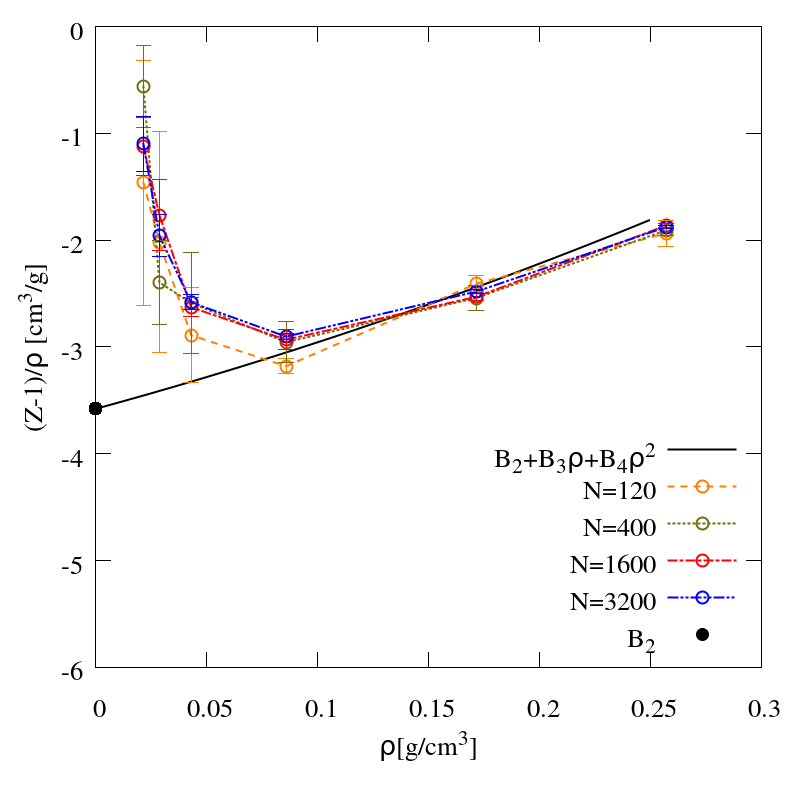
\includegraphics[scale=0.3]{Figures/FSE_TraPPE-C2_Lammps-flex_IT.png}
\caption{Effect of number of ethane molecules on compressibility factor at low densities in MD simulation ($T^{\mathrm{IT}}=360 \, \mathrm{K}$). State points are simulated in LAMMPS with flexible C-C bonds. The bond constant was obtained from Nath et al.  \cite{Nath1998a}. The simulations were run using multiple-time-step algorithm RESPA \cite{tuckerman1992}. 
}
\label{fig:FSE_TraPPE_C2_Lammps_flex_IT}
\end{figure}

\begin{figure}
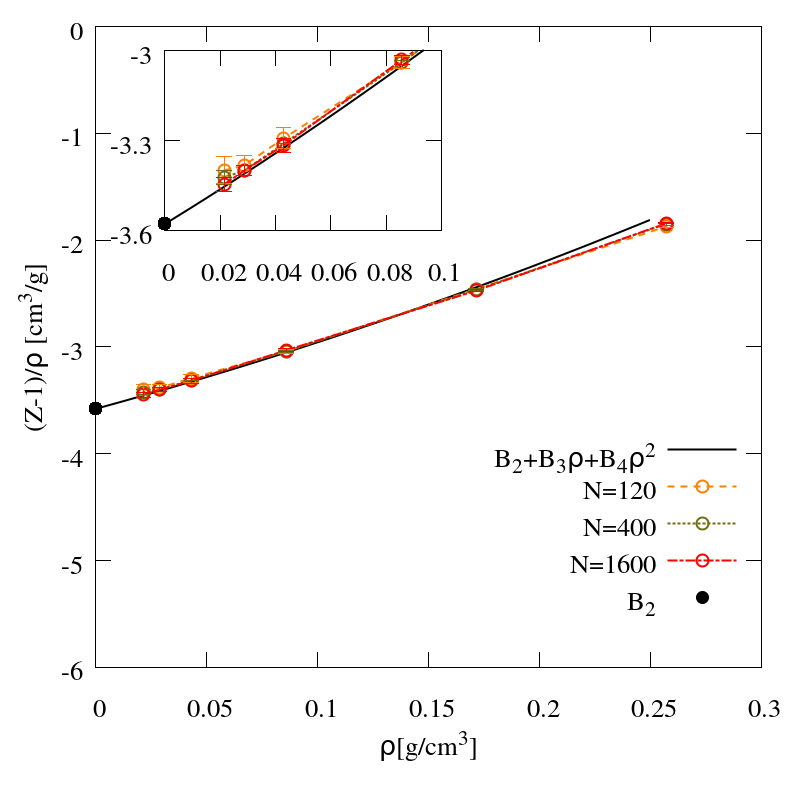
\includegraphics[scale=0.3]{Figures/FSE_TraPPE-C2_GOMC_IT.png}
\caption{Effect of number of ethane molecules on compressibility factor at low densities in MC simulation ($T^{\mathrm{IT}}=360 \, \mathrm{K}$). State points are simulated in GOMC.}
\label{fig:FSE_TraPPE_C2_GOMC_IT}
\end{figure}


\section{Simulation Details} \label{sec:SimDetail}
In principle, both Monte Carlo and molecular dynamics methods can be used to simulate the $NVT$ state points required to construct the isothermal and isochoric paths in the ITIC method. In this study, the MC method with fixed bond lengths was favored due to lower fluctuations. The Cassandra package \cite{Shah2017} was used to simulate ethane and \textit{n}-dodecane systems in the $NVT$ ensemble using the TraPPE-UA potential model. In united-atom force fields, interaction sites may consist of a group of atoms, which is centered on the main atom of the group for the TraPPE-UA method \cite{Smit1998}. In TraPPE-UA model van der Waals interactions are truncated at $14\,\mathrm{\AA}$ and standard analytical long-range corrections are applied to compensate for truncation effects on energy and pressure\cite{allen2017}. In TraPPE-UA, the bond lengths are considered fixed and the bond energy is zero. This approximation results in less pressure fluctuation at low densities, but we note that the MC results at high densities were consistent with MD results simulated in LAMMPS \cite{Plimpton2007} within their uncertainties.

Packmol \cite{martinez2009packmol} package was used to create the initial configurations. The simulation boxes contained 1200 sites except for the four simulations required for estimating $B_2$ at isotherm temperature (the purple and green points in Fig.~\ref{fig:ITICpathway}) for which simulation boxes contained 4800 sites. Standard Periodic Boundary Conditions (PBCs) was used. Simulations were run for 30 million Monte Carlo steps (MCS), and the last 15 million MCS were used for calculating the properties which were stored every 50,000 MC steps. For each compound, 22 $NVT$ points were simulated in order to obtain 5 saturation points as illustrated in Fig.~\ref{fig:ITICpathway}. The density of the isochore with highest density was picked to match the experimental liquid density at the minimum reduced saturation temperature ($T_r^{min}$) of 0.45. Isothermal reduced temperatures for ethane and \textit{n}-dodecane were 1.18 and 1.05, respectively. Density and temperature of simulated state points for all simulated compounds are listed in supplementary material along with pressure and energies averages from Cassandra simulation at each point.

\subsection{Internal Energy Departure Function Calculation}\label{sec:udepCalc}
The internal energy departure function in Eq.~(\ref{eqn:eqn8}) was calculated for isochoric points using Eq.~(\ref{eqn:uDepForm})

\begin{equation}
U^{\mathrm{dep}} = \frac{E^{\mathrm{tot}} - E^{\mathrm{bonded}} - E^{\mathrm{intra}}}{NRT}\label{eqn:uDepForm}
\end{equation}
where $E^{\mathrm{tot}}$, $E^{\mathrm{bonded}}$, and $E^{\mathrm{intra}}$ are the total potential energy, bonded energy (bond, angle, and dihedral), and intramolecular pairwise energy (coulumbic and van der Waals). $N$ represents the number of molecules in the simulation box, $R$ is the gas constant ($8.3144598\,\mathrm{J/(mol.K)}$), and $T$ represents the temperature. Failing to subtract $E^{\mathrm{intra}}$ causes a significant error in vapor pressure. A post-processing code is required to calculate this quantity, if the molecular simulation package does not provide an internal way of estimating it (e.g. LAMMPS). In this case it is necessary to output the site coordinates a few times during the simulation.

\subsection{Bootstraping Method for Uncertainty Calculation}\label{sec:bootstrapping}
Bootstrapping was used to calculate the statistical uncertainties \cite{Efron1981}. Four series of independent $NVT$ simulations were performed for each compound using different random number generator seeds. The $NVT$ state points required for ITIC analysis were then randomly selected from the four series of $NVT$ state points. This process was repeated 500 times and ITIC analysis was performed each time on the resulting set of randomly selected $NVT$ points. The standard deviations were then calculated from the resulting 500 ITIC outputs. 
%RAM: We need to be more clear as to what uncertainties we are representing in Figures and Tables. I assume they are standard deviations. But if they are 95\% confidence intervals then this statement will need to be modified.
The bootstrap standard deviations are represented in Fig.~\ref{fig:EXAMPLE-SIM/TraPPE-C2/Psat}-\ref{fig:EXAMPLE-SIM/Mie-C12/T_rho} and provided in Tables~\ref{tab:EXAMPLE-SIM/TraPPE-C2}-\ref{tab:EXAMPLE-SIM/Mie-C12/}. 
%RAM: 5/3 I think we just want to mention that uncertainties are found for Tsat, Psat, etc. not for rhol
Note that the ITIC method determines saturation conditions at a fixed value of $\rho_{\mathrm{liq}}$ (equal to the isochoric density) and, therefore, the bootstrap uncertainty in $\rho_{\mathrm{liq}}$ is zero.

\subsection{Critical Pressure Calculation}\label{sec:PcCalc}
The critical temperatures and densities can be estimated by the law of rectilinear diameter \cite{Rowlinson1982} and the density scaling law \cite{Rowlinson2013} for critical temperature

\begin{equation}
\frac{\rho_{\mathrm{liq}} +\rho_{\mathrm{vap}}}{2}=\rho_c+A(T_c-T)
\label{eqn:rectilinearLaw}
\end{equation}

\begin{equation}
\rho_{\mathrm{liq}} -\rho_{\mathrm{vap}}=B(T_c-T)^{0.325}
\label{eqn:scalingLaw}
\end{equation}
where $A$ and $B$ are constants that are fit to simulation data.

Critical pressure and acentric factor were calculated by plugging critical temperature obtained from Eq.~(\ref{eqn:rectilinearLaw}) and Eq.~(\ref{eqn:scalingLaw}) into Lee-Kesler equation \cite{Lee1975} and fitting vapor pressure and saturation temperatures.
			
\begin{equation}
{\ln \frac{P}{P_c}=f^{(0)}+\omega f^{(1)}} 
\label{eqn:Lee-Kesler}
\end{equation}
where $P_c$ and $\omega$ represent critical pressure and acentric factor, respectively. $f^{(0)}$ and $f^{(1)}$ terms are defined in Eq.~(\ref{eqn:Lee-Kesler-terms})
\begin{equation}
\begin{array}{l} 
{f^{(1)} = 15.2518 - \frac{15.6875}{T_r} - 13.4721 \, \ln(T_r) +   0.43577 \, T_r^6 } \\ 
{ f^{(0)} = 5.92714 - \frac{6.09648}{T_r} - 1.28862 \, \ln(T_r) + 0.169347 \, T_r^6  } 
\end{array} \label{eqn:Lee-Kesler-terms}
\end{equation}
	
%RAM: Enthalphy of vaporization is less ambiguous than heat of vaporization	
\subsection{Enthalpy of Vaporization Calculation}\label{sec:HvapCalc}
In ITIC method, enthalpy of vaporization ($\Delta H_\mathrm{v}$) is calculated using Eq.~(\ref{eqn:Hvap})
%RAM: We should not use DeltaH_vap if we use "vap" to mean vapor, not vaporization. Changing this to DeltaH_v
\begin{equation}
\Delta H_\mathrm{v}= ( H^{\mathrm{dep,sat}}_\mathrm{vap} - H^{\mathrm{dep,sat}}_\mathrm{liq})RT
\label{eqn:Hvap}
\end{equation}
where $R$ is gas constant and $H^{\mathrm{dep}}$ is defined as
\begin{equation}
H^{\mathrm{dep}}=\frac{H-H^{\mathrm{ig}}}{RT}
\label{hdep}
\end{equation}
$H^{\mathrm{dep,sat}}_\mathrm{vap}$ and $H^{\mathrm{dep,sat}}_\mathrm{liq}$ are unitless enthalpy departure functions of saturated vapor and liquid, respectively, which can be calculated by subtracting the ideal gas contribution from both sides of $H=U+PV$

\begin{equation}
H^{\mathrm{dep,sat}}_\mathrm{liq} \approx U^{\mathrm{dep, sat}}_\mathrm{liq}+Z_\mathrm{liq} - 1
\label{eqn:HsatLiq}
\end{equation}

\begin{equation}
H^{\mathrm{dep,sat}}_\mathrm{vap} \approx U^{\mathrm{dep, sat}}_\mathrm{vap}+Z_\mathrm{vap} - 1
\label{eqn:HsatVap}
\end{equation}

The value of $U^{\mathrm{dep, sat}}_\mathrm{liq}$, as explained in Section~\ref{sec:ITIC-method}, is calculated at each fixed-point iteration based on the updated value of $T^{\mathrm{sat}}$. According to Eq.~\ref{eqn:b2uDep}, the value of $U^{\mathrm{dep, sat}}_\mathrm{vap}$ is approximated by taking the derivative of $B_2$ with respect to $\beta$ as shown in Eq.~(\ref{eqn:dB2dbeta}).
\begin{equation}
U^{\mathrm{dep, sat}}_\mathrm{vap}\approx \rho_{\mathrm{vap}} \beta \frac{dB_2}{d\beta} \approx \frac{\rho_{\mathrm{vap}}}{T^{\mathrm{sat}}} \frac{B_2^{\mathrm{sat}}-B_2^{\mathrm{IT}}}{\frac{1}{T^{\mathrm{sat}}} - \frac{1}{T^{\mathrm{IT}}}}
\label{eqn:dB2dbeta}
\end{equation}

\section{Example Simulations} \label{sec:ExampleSim}
The TraPPE-UA \cite{Martin1998,Martin1999,Wick2000}, Mie-UA \cite{Potoff2009,Mick2017,Barhaghi2017,Mick2015}, and TITP4P/2005 \cite{Abascal2005} models were chosen for the purpose of testing the ITIC method due to the availability of literature simulation results \cite{Martin1998,eggimann2014,Potoff2009,Shen2008}. As mentioned in Section~\ref{sec:SimDetail}, pure ethane and \textit{n}-dodecane systems were simulated using Cassandra package \cite{Shah2017} in the canonical ensemble to obtain the $NVT$ state points. The saturation points calculated using the ITIC method were then compared against TraPPE-UA results obtained using Gibbs Ensemble Monte Carlo method (GEMC) which are available from the TraPPE website.\cite{eggimann2014} Fig.~\ref{fig:EXAMPLE-SIM/TraPPE-C2/Psat}-\ref{fig:EXAMPLE-SIM/TraPPE-C2/T_rho} show this comparison for ethane and Fig.~\ref{fig:EXAMPLE-SIM/TraPPE-C12/Psat}-\ref{fig:EXAMPLE-SIM/TraPPE-C12/T_rho} provide this information for \textit{n}-dodecane. The isothermal/isochoric plots of $A^{\mathrm{dep}}$, $U^{\mathrm{dep}}$, $Z$, $\Delta H_{\mathrm{v}}$, and $B_2$ for all example simulations are included in supplementary material. 
%RAM: Included statement about uncertainties being from bootstrapping
%RAM: 5/3 Removed deviations from NIST REFPROP
%RAM: 5/3 Also included clarification for why rhol does not have an uncertainty
%RAM: 5/3 I decided to move this statement to the section on bootstrapping. This was what I had before:
%Note that each $\rho_{\mathrm{liq}}$ value is equal to the corresponding isochoric density and, therefore, the ITIC uncertainty in $\rho_{\mathrm{liq}}$ is zero.
\begin{table*}[]
\centering
\caption{ITIC method saturation properties and uncertainties for ethane using TraPPE-UA model. Virial expansion was truncated at $B_2$. ITIC uncertainties correspond to bootstrap standard deviations.}
\label{tab:EXAMPLE-SIM/TraPPE-C2}
\begin{ruledtabular}
\begin{tabular}{cccccccccccccccccccccccc}
 & \multicolumn{2}{c}{$[\mathrm{K}]$} &	 \multicolumn{2}{c}{$[\mathrm{MPa}]$} & $[\mathrm{g/cm^3}]$ & \multicolumn{2}{c}{$[\mathrm{g/cm^3}]$} & \multicolumn{2}{c}{$[\mathrm{kJ/mol}]$} \\
$T_r^{\mathrm{sat}}$ & $T^{\mathrm{sat}}$ & $\pm$ & $P^{\mathrm{sat}}$ & $\pm$ & $\rho_{\mathrm{liq}}$ & $\rho_{\mathrm{vap}}$ & $\pm$ & $\Delta H_{\mathrm{v}}$ & $\pm$
 \\
\hline		
0.85	&	259.66	&	0.88	&	2.03290	&	0.04847		&	0.4286	&	0.038454	&	0.001116	&	9.587	&	0.041	\\
0.77	&	235.00	&	1.33	&	1.03560	&	0.04182		&	0.4714	&	0.018879	&	0.000761	&	11.243	&	0.027	\\
0.67	&	205.72	&	0.32	&	0.37902	&	0.00524		&	0.5143	&	0.007212	&	0.000096	&	12.626	&	0.003	\\
0.57	&	173.57	&	0.30	&	0.08321	&	0.00147		&	0.5571	&	0.001780	&	0.000029	&	13.804	&	0.002	\\
0.45	&	138.20	&	0.28	&	0.00632	&	0.00017		&	0.6000	&	0.000166	&	0.000004	&	14.868	&	0.003	\\
\end{tabular}
\end{ruledtabular}
\end{table*}





\begin{figure}
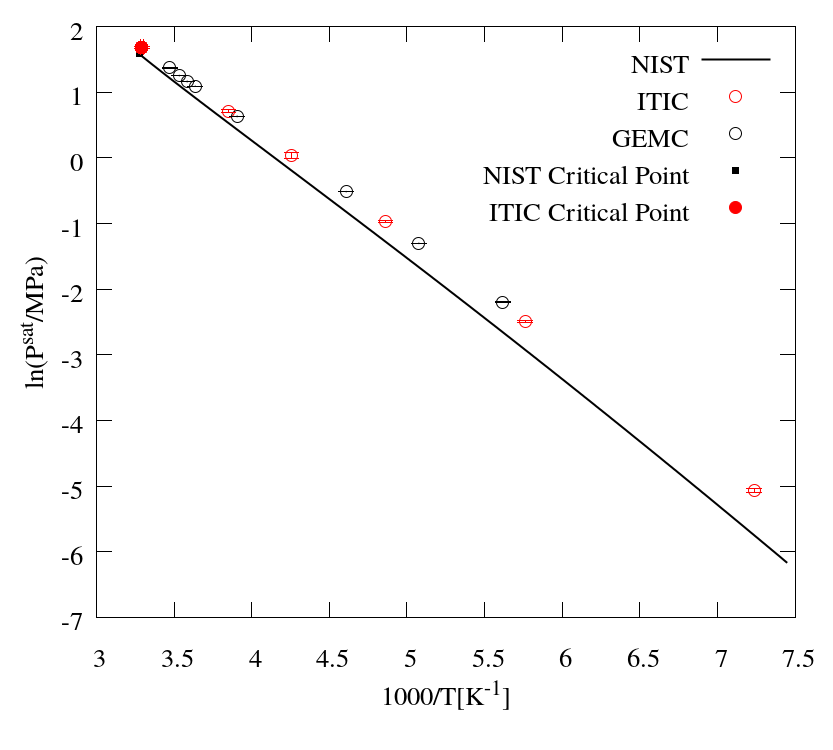
\includegraphics[scale=0.30]{Figures/EXAMPLE-SIM_TraPPE-C2_psat.png}
\caption{$P^{\mathrm{sat}}$ plot of TraPPE-UA ethane. The virial expansion shown in Eq.~(\ref{eqn:eqn11}) was truncated at the $B_2$ term. GEMC data were obtained from Ref.~\onlinecite{Martin1998}.}
\label{fig:EXAMPLE-SIM/TraPPE-C2/Psat}
\end{figure}

\begin{figure}
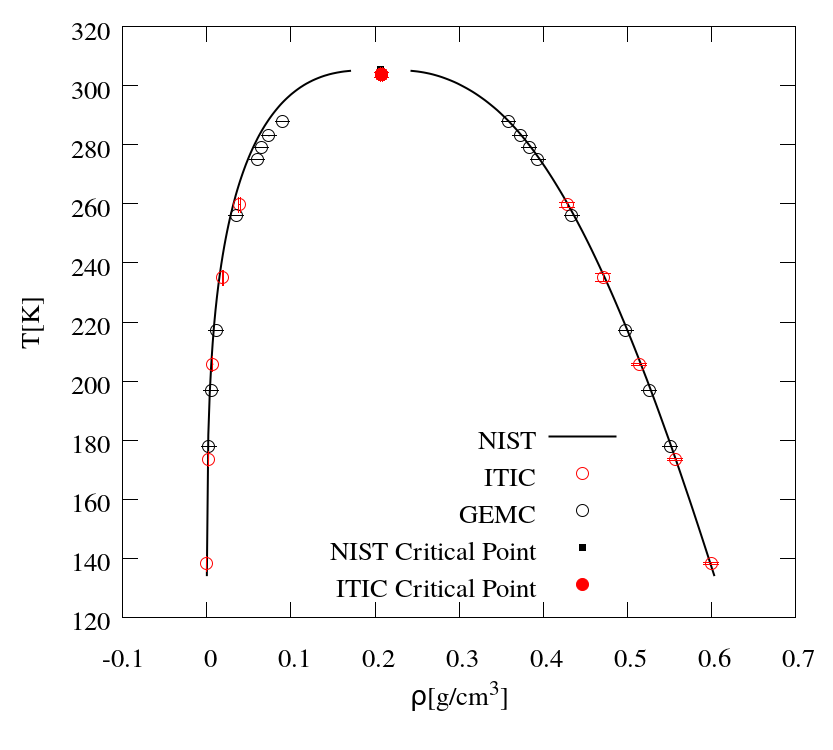
\includegraphics[scale=0.30]{Figures/EXAMPLE-SIM_TraPPE-C2_trho.png}
\caption{Coexistence curves for TraPPE-UA ethane. The virial expansion shown in Eq.~(\ref{eqn:eqn11}) was truncated at the $B_2$ term. GEMC data were obtained from Ref.~\onlinecite{Martin1998}.}
\label{fig:EXAMPLE-SIM/TraPPE-C2/T_rho}
\end{figure}

\begin{table*}[]
\centering
\caption{ITIC method saturation properties and uncertainties for \textit{n}-dodecane using TraPPE-UA model. Virial expansion was truncated at $B_2$. ITIC uncertainties correspond to bootstrap standard deviations.}
\label{tab:EXAMPLE-SIM/TraPPE-C12}
\begin{ruledtabular}
\begin{tabular}{cccccccccccccccccccccccc}
 & \multicolumn{2}{c}{$[\mathrm{K}]$} &	 \multicolumn{2}{c}{$[\mathrm{MPa}]$} & $[\mathrm{g/cm^3}]$ & \multicolumn{2}{c}{$[\mathrm{g/cm^3}]$} & \multicolumn{2}{c}{$[\mathrm{kJ/mol}]$} \\
$T_r^{\mathrm{sat}}$ & $T^{\mathrm{sat}}$ & $\pm$ & $P^{\mathrm{sat}}$ & $\pm$ & $\rho_{\mathrm{liq}}$ & $\rho_{\mathrm{vap}}$ & $\pm$ & $\Delta H_{\mathrm{v}}$ & $\pm$
 \\
\hline													
0.85	&	556.30	&	3.97	&	0.47993	&	0.037368	&	0.5336	&	0.021841	&	0.0019474	&	33.733	&	0.280	\\
0.77	&	503.62	&	1.99	&	0.18021	&	0.009544	&	0.5870	&	0.008069	&	0.0004412	&	39.463	&	0.081	\\
0.68	&	446.81	&	1.14	&	0.04585	&	0.002087	&	0.6404	&	0.002177	&	0.0000986	&	44.564	&	0.032	\\
0.57	&	376.92	&	0.95	&	0.00419	&	0.000210	&	0.6937	&	0.000229	&	0.0000111	&	49.517	&	0.021	\\
0.46	&	305.16	&	0.68	&	0.00008	&	0.000005	&	0.7471	&	0.000005	&	0.0000003	&	54.757	&	0.008	\\				
\end{tabular}
\end{ruledtabular}
\end{table*}

\begin{table*}[]
\centering
\caption{ITIC method saturation properties and uncertainties for \textit{n}-dodecane using Mie-UA model. Virial expansion was truncated at $B_2$. ITIC uncertainties correspond to bootstrap standard deviations.}
\label{tab:EXAMPLE-SIM/Mie-C12/}
\begin{ruledtabular}
\begin{tabular}{cccccccccccccccccccccccc}
 & \multicolumn{2}{c}{$[\mathrm{K}]$} &	 \multicolumn{2}{c}{$[\mathrm{MPa}]$}	& $[\mathrm{g/cm^3}]$ & \multicolumn{2}{c}{$[\mathrm{g/cm^3}]$} & \multicolumn{2}{c}{$[\mathrm{kJ/mol}]$} \\
$T_r^{\mathrm{sat}}$ & $T^{\mathrm{sat}}$ & $\pm$ & $P^{\mathrm{sat}}$ & $\pm$ & $\rho_{\mathrm{liq}}$ & $\rho_{\mathrm{vap}}$ & $\pm$ & $\Delta H_{\mathrm{v}}$ & $\pm$
 \\
\hline													
0.84	&	550.30	&	3.95	&	0.37071	&	0.030178	&	0.5336	&	0.016258	&	0.0014257	&	38.433	&	0.270	\\
0.76	&	499.12	&	2.59	&	0.12778	&	0.008755	&	0.5870	&	0.005632	&	0.0003811	&	44.633	&	0.106	\\
0.66	&	435.23	&	1.14	&	0.02235	&	0.001169	&	0.6404	&	0.001073	&	0.0000548	&	50.447	&	0.051	\\
0.56	&	368.28	&	2.15	&	0.00146	&	0.000158	&	0.6937	&	0.000081	&	0.0000084	&	56.281	&	0.029	\\
0.45	&	294.97	&	1.99	&	0.00001	&	0.000002	&	0.7471	&	0.000001	&	0.0000001	&	62.700	&	0.037	\\
\end{tabular}
\end{ruledtabular}
\end{table*}

\begin{table*}[]
\centering
\caption{ITIC method saturation properties for water using TIP4P/2005 model. Virial expansion was truncated at $B_2$. ITIC uncertainties are not reported due to high computational cost of replicate simulations.}
\label{tab:EXAMPLE-SIM/TIP4P-water}
\begin{ruledtabular}
\begin{tabular}{cccccc}
 & {[}K{]} &	 {[}MPa{]} & {[}$\mathrm{g/cm^3}${]} & {[}$\mathrm{g/cm^3}${]}	& {[}kJ/mol{]}  \\
$T_r^{\mathrm{sat}}$ & $T^{\mathrm{sat}}$ & $P^{\mathrm{sat}}$ & $\rho_{\mathrm{liq}}$ & $\rho_{\mathrm{vap}}$ & $\Delta H_{\mathrm{v}}$ \\
\hline													
0.87	&	563.50	&	4.30448	&	0.7129	&	0.020456	&	33.56	\\
0.81	&	526.26	&	2.32442	&	0.7841	&	0.011181	&	36.64	\\
0.73	&	471.35	&	0.74423	&	0.8554	&	0.003659	&	40.57	\\
0.63	&	405.95	&	0.11965	&	0.9267	&	0.000651	&	44.47	\\
0.47	&	301.91	&	0.00093	&	0.9980	&	0.000007	&	49.98	\\
\end{tabular}
\end{ruledtabular}
\end{table*}




\begin{figure}
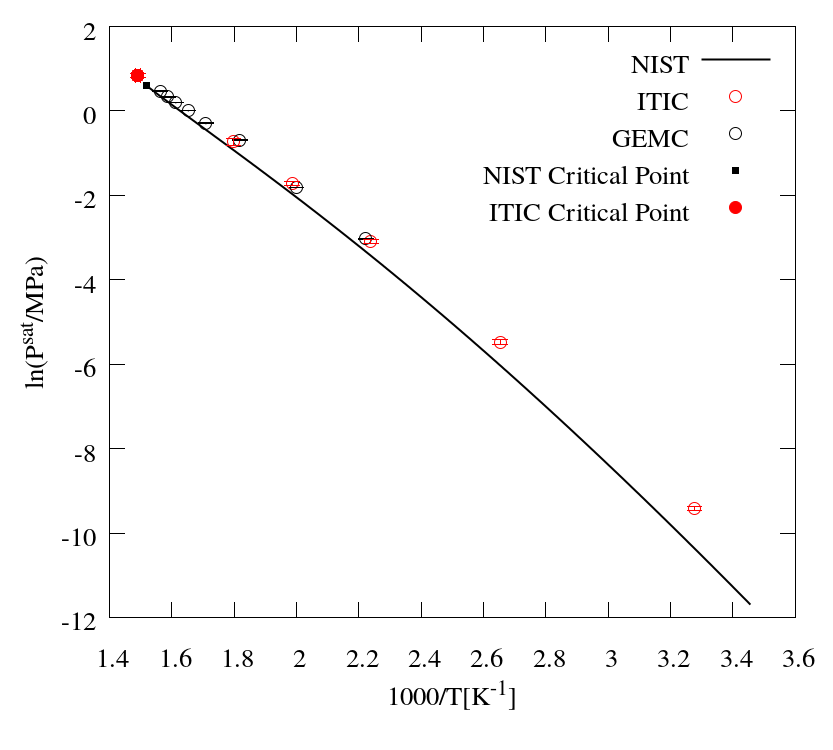
\includegraphics[scale=0.30]{Figures/EXAMPLE-SIM_TraPPE-C12_psat.png}
\caption{$P^{\mathrm{sat}}$ plot of TraPPE-UA \textit{n}-dodecane. The virial expansion shown in Eq.~(\ref{eqn:eqn11}) was truncated at the $B_2$ term. GEMC data were obtained from Ref.~\onlinecite{Martin1998}.}
\label{fig:EXAMPLE-SIM/TraPPE-C12/Psat}
\end{figure}

\begin{figure}
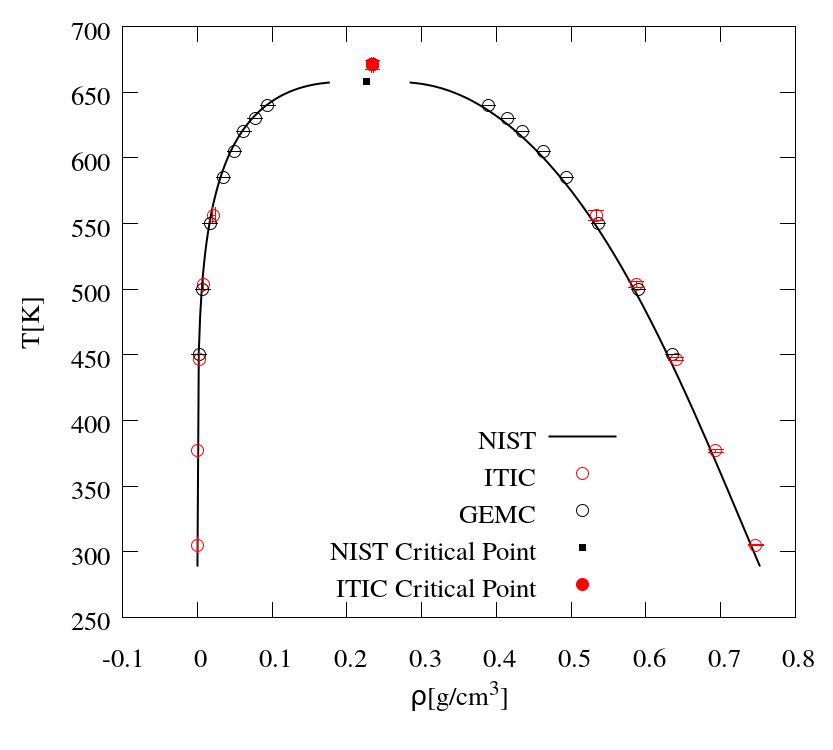
\includegraphics[scale=0.30]{Figures/EXAMPLE-SIM_TraPPE-C12_trho.png}
\caption{Coexistence curves for TraPPE-UA \textit{n}-dodecane. The virial expansion shown in Eq.~(\ref{eqn:eqn11}) was truncated at the $B_2$ term. GEMC data were obtained from Ref.~\onlinecite{Martin1998}.}
\label{fig:EXAMPLE-SIM/TraPPE-C12/T_rho}
\end{figure}


The ITIC method was also compared to histogram-reweighting Monte Carlo in the grand canonical ensemble (GCMC). \textit{n}-Dodecane was simulated with Cassandra using Mie-UA potential parameters \cite{Potoff2009}. GCMC results in Fig.~\ref{fig:EXAMPLE-SIM/Mie-C12/Psat} and Fig.~\ref{fig:EXAMPLE-SIM/Mie-C12/T_rho} are not available below a minimum reduced temperature ($T_r^{\mathrm{min}}$) of 0.67, however the ITIC method allowed us to calculate vapor pressure and liquid densities densities for reduced temperatures as low as 0.45. In this simulation $B_3$ was not used and a $B_2$ correlation was obtained using the method described in Section~\ref{sec:VirialCalc}. Fig.~\ref{fig:EXAMPLE-SIM/Mie-C12/Z_rho} shows the supercritical isotherm and the state points used for $B_2$ calculation.

\begin{figure}
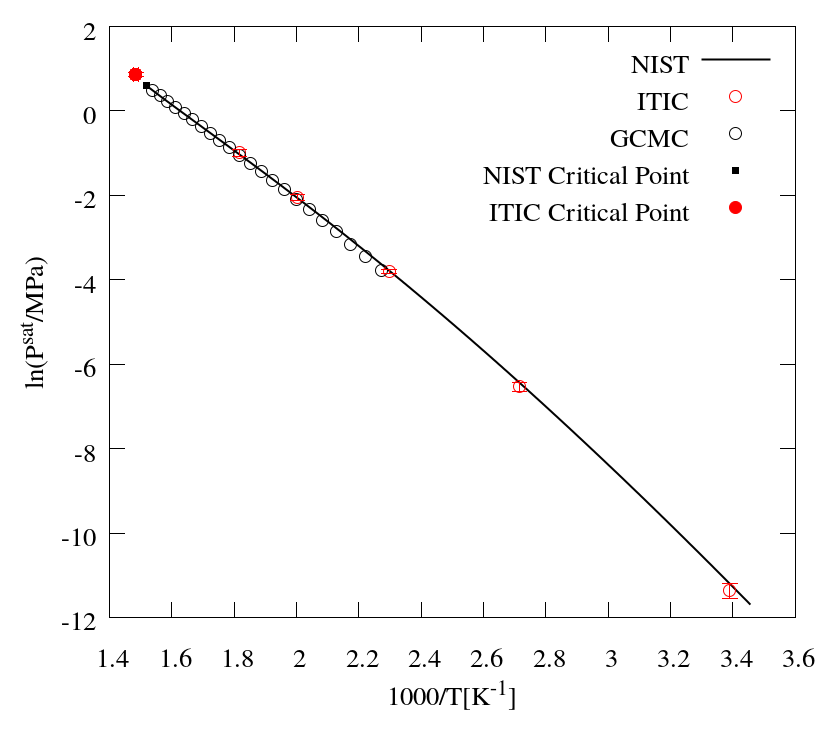
\includegraphics[scale=0.30]{Figures/EXAMPLE-SIM_Mie-C12_psat.png}
\caption{Clausius-Clapeyron plot of Mie-UA \textit{n}-dodecane. GCMC data were obtained from Potoff's work\cite{Potoff2009}.}
\label{fig:EXAMPLE-SIM/Mie-C12/Psat}
\end{figure}

\begin{figure}
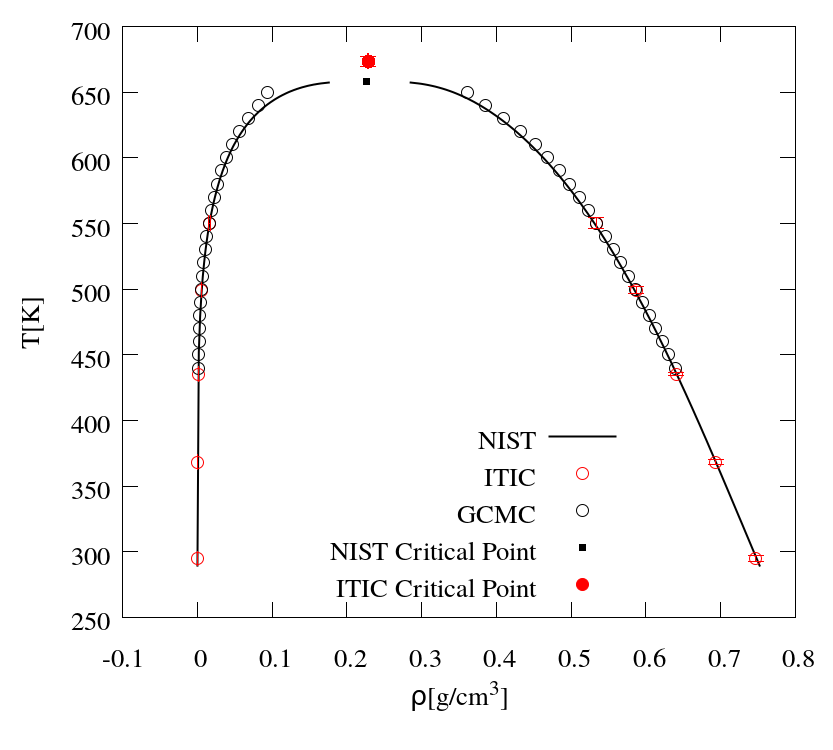
\includegraphics[scale=0.30]{Figures/EXAMPLE-SIM_Mie-C12_trho.png}
\caption{Coexistence curves for Mie-UA \textit{n}-dodecane. GCMC data were obtained from Potoff's work\cite{Potoff2009}.}
\label{fig:EXAMPLE-SIM/Mie-C12/T_rho}
\end{figure}

\begin{figure}
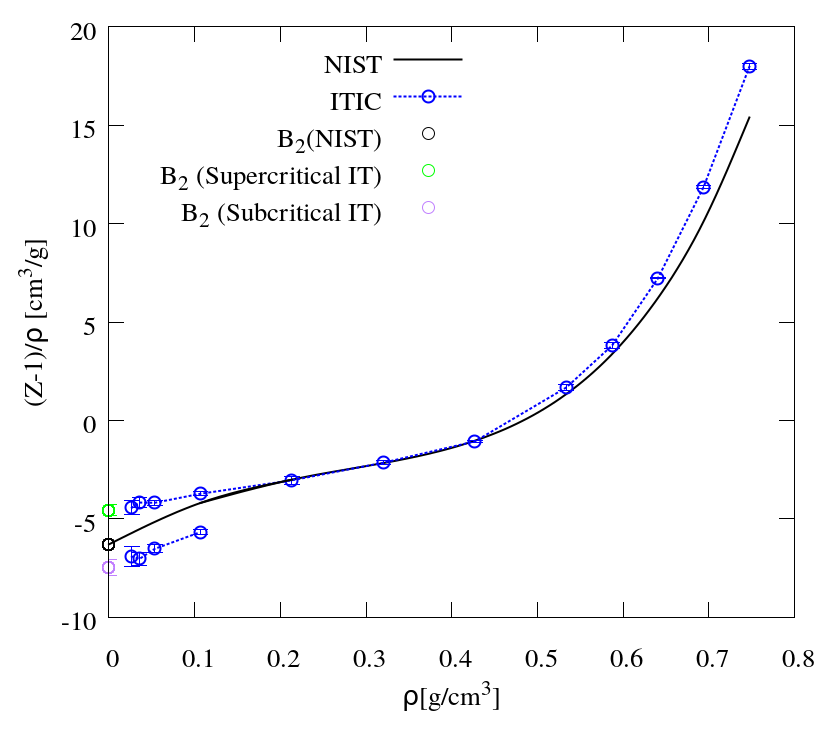
\includegraphics[scale=0.30]{Figures/EXAMPLE-SIM_Mie-C12_zrho.png}
\caption{Compressibility factor plot of Mie-UA \textit{n}-dodecane. The lower isotherm was simulated to calculate the purple point, i.e. the $B_2$ value at $T_r=0.9$.}
\label{fig:EXAMPLE-SIM/Mie-C12/Z_rho}
\end{figure}



In order to validate the ITIC method for polar molecules, the results of the ITIC method using TIP4P/2005 water simulated in Cassandra were compared against TIP4P/2005 data from NIST Standard Reference Simulation \cite{Shen2008} simulated using grand-canonical Wang-Landau/Transition-matrix Monte Carlo and histogram re-weighting. Fig.~\ref{fig:EXAMPLE-SIM/TIP4P05/Psat} and Fig.~\ref{fig:EXAMPLE-SIM/TIP4P05/T_rho} shows the agreement between the two methods for TIP4P/2005 water. The absolute average deviation percent between vapor pressure calculated using ITIC method and NIST simulation data for TIP4P/2005 water shown in Fig.~\ref{fig:EXAMPLE-SIM/TIP4P05/Psat} is less than 3 \%. 


\begin{figure}
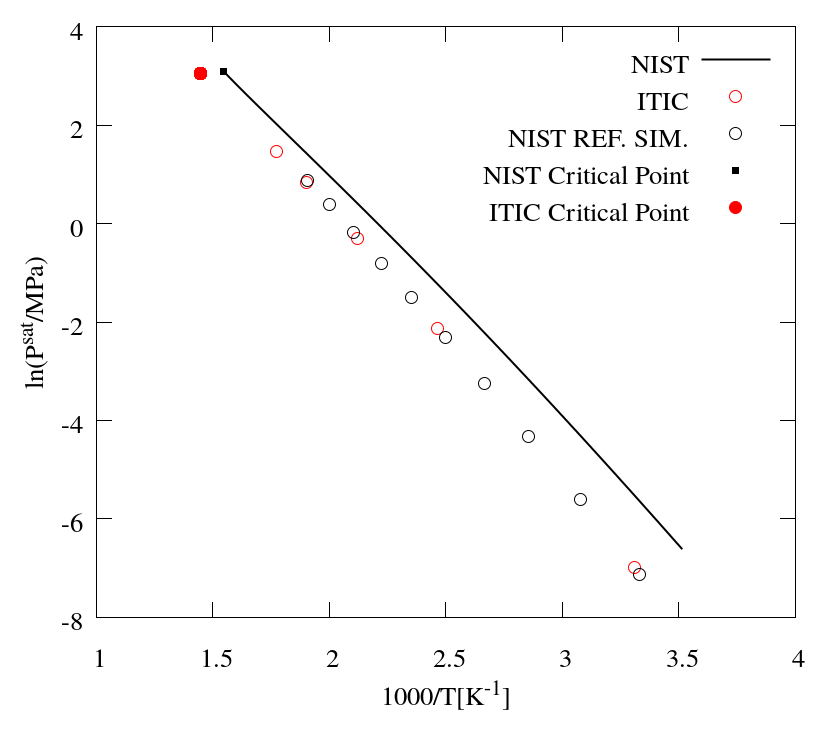
\includegraphics[scale=0.30]{Figures/EXAMPLE-SIM_TIP4P05_psat.png}
\caption{Clausius-Clapeyron plot of TIP4P/2005 water. GCMC data were obtained from NIST Standard Reference Simulation website \cite{Shen2008}. $B_2$ values at saturation temperatures were obtained from Benjamin et al.\cite{Benjamin2007} and Chiavo et al. \citep{Chialvo2006}. }
\label{fig:EXAMPLE-SIM/TIP4P05/Psat}
\end{figure}

\begin{figure}
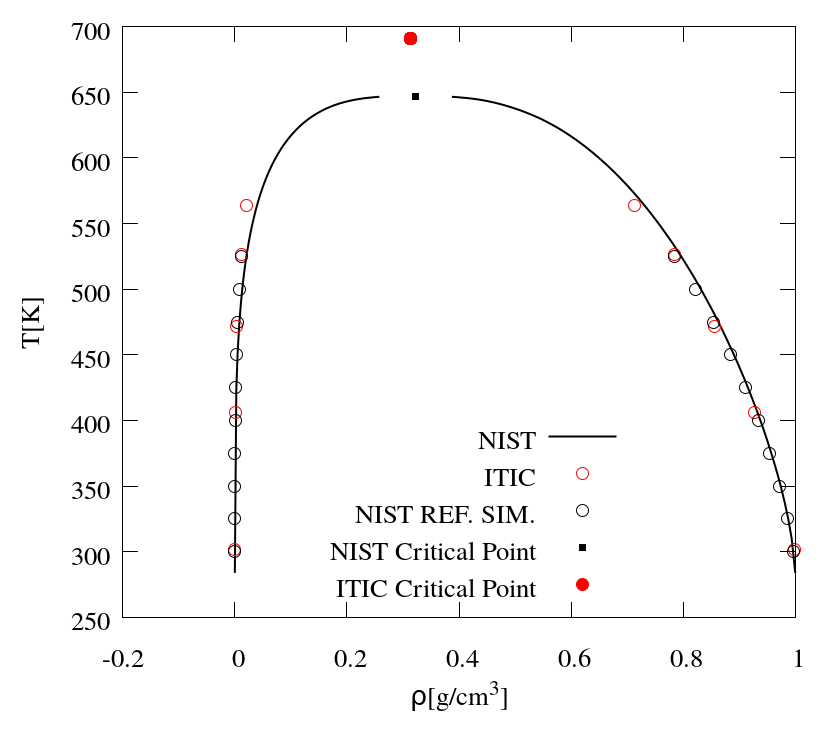
\includegraphics[scale=0.30]{Figures/EXAMPLE-SIM_TIP4P05_trho.png}
\caption{Coexistence curves for TIP4P/2005 water. GCMC data were obtained from NIST Standard Reference Simulation website \cite{Shen2008}.}
\label{fig:EXAMPLE-SIM/TIP4P05/T_rho}
\end{figure}



\section{Conclusions} \label{sec:conclusion} 
Isothermal-isochoric integration method (ITIC) was shown to be a reliable alternative for phase equilibrium calculations. Validation against NIST REFPROP values showed that, in the absence of simulation uncertainty, the vapor pressure calculated by ITIC method with 9 points on IT and 3 points on IC sufficed to reproduce NIST REFPROP vapor pressure within 0.2 \% deviation. ITIC is sensitive to low density $NVT$ simulations and the noise issue at low densities can be addressed by simulating larger systems, and preferring MC methods with fixed bond lengths when feasible.

It is important for engineering applications to be able to simulate systems at temperatures as low as $T_r=0.45$ \cite{Reid1987}. Monte Carlo methods such as GEMC and GCMC usually have a minimum reduced temperature limit of about 0.6 \cite{Martin1998}. The ITIC method, hence, outperforms GEMC and GCMC when $T_r$ is less than 0.6. This method, on the other hand, is less favorable at high reduced temperatures, especially above $T_r=0.85$, mostly due to lack of a convenient method to characterize the virial coefficients. MC methods can be used when the temperature is above $T_r=0.6$, but if applications below 0.6 are of prospective interest, then MC methods lose their efficiency advantage, because in ITIC  method, the entire isotherm must be generated. 

In conclusion, it is recommended to approach the problem of coexistence calculation with a combination of Monte Carlo (GEMC or GCMC) and isothermal-isochoric  integration in order to cover the entire range of industrially relevant temperatures. If a single method is preferred, or if MD is the preferred simulation method, ITIC can easily be implemented from $T_r = 0.85$ to $0.45$ with less than 50 \% additional computational time requirement over the combined method.

%%%RAM 4/23/18: This section is required for all NIST employees
\section{Acknowledgments}

This research was performed while R.A.M. held a National Research Council (NRC) Postdoctoral Research Associateship at the National Institute of Standards and Technology (NIST). Contribution of NIST, an agency of the United States government; not subject to copyright in the United States.
%%%

\section{Supplementary Material} \label{sec:SupMat} 
See supplementary material for density, temperature, $Z$ and energies of simulated state points for all simulated compounds, as well as the isothermal/isochoric plots of $A^{\mathrm{dep}}$, $U^{\mathrm{dep}}$, $Z$, $\Delta H_{\mathrm{v}}$, and $B_2$ for all example simulations. 

\section{References} \label{sec:ref} 
\bibliography{ITIC-Paper}
\end{document}
